\documentclass[10pt,a4paper]{ctexart}

% 页面设置
\usepackage[top=2.5cm, bottom=2.5cm, left=2.5cm, right=2.5cm]{geometry}

% 数学与符号
\usepackage{amsmath,amssymb,amsfonts}
\usepackage{bm}

% 图表
\usepackage{graphicx}
\usepackage{booktabs}
\usepackage{multirow}
\usepackage{subcaption}
\usepackage{array}
\usepackage{float}

% 颜色与链接
\usepackage{xcolor}
\usepackage{hyperref}
\hypersetup{
    colorlinks=true,
    linkcolor=blue,
    filecolor=magenta,
    urlcolor=cyan,
    citecolor=blue
}

% 算法
\usepackage{algorithm}
\usepackage{algorithmic}
\floatname{algorithm}{算法}
\renewcommand{\algorithmicrequire}{\textbf{输入：}}
\renewcommand{\algorithmicensure}{\textbf{输出：}}

% 代码与引用
\usepackage{listings}
\usepackage[numbers,sort&compress]{natbib}

% 其他
\usepackage{url}
\usepackage{enumitem}
\usepackage{threeparttable}

% 图片路径
\graphicspath{{figures/}}

% 标题信息
\title{\textbf{基于缺失指示器的电池健康状态预测方法对比研究：\\XJTU数据集上的深度学习模型与多缺失率实验}}
\author{作者姓名$^{1}$ \quad 通讯作者$^{2}$}
\date{$^{1}$作者单位 \\ $^{2}$通讯作者单位 \\ \texttt{email@example.com}}

\begin{document}

\maketitle

%==============================================================================
\begin{abstract}
锂离子电池健康状态（State of Health, SOH）的准确预测对于保障电动汽车和储能系统的安全可靠运行具有至关重要的意义。然而，在实际工程应用中，由于传感器故障、通信中断、数据采集异常等多种因素，电池监测数据普遍存在不同程度的缺失问题。传统的缺失数据处理方法通常将缺失视为噪声需要修复，而忽略了"哪些信息缺失"本身可能包含的有用信号，这在高缺失率场景下尤其限制了预测模型的性能上限。

本文以公开的XJTU锂离子电池数据集为研究对象，引入实现简单的缺失指示器方法（Missing Indicator Method, MIM），系统评估其在多种常用模型架构和不同缺失率条件下对SOH预测性能与鲁棒性的影响。在数据预处理阶段，我们以循环为样本单位提取16个循环级统计特征，构建循环级SOH标签；在缺失模拟阶段，通过随机方式在特征层面注入九档缺失率（Missing Rate, MR）$\{0.1, 0.2, \ldots, 0.9\}$，采用均值插补方法填补缺失值；在特征增强阶段，为每个特征构造二值缺失指示器，将"插补值与指示器拼接"作为MIM输入。我们选取了MLP、LSTM、GRU与1D-CNN四种代表性深度学习模型，在PyTorch 2.5.1深度学习框架下统一训练和评估，对比分析"仅插补"和"MIM输入"两类策略在不同缺失率下的SOH预测误差与鲁棒性差异。

实验结果表明，在缺失率$\geq 0.4$条件下，引入缺失指示器的MIM版本在四种神经网络模型中均显著降低SOH预测误差（改进率50\%--96\%）。具体而言，在MR=0.5时，1D-CNN-MIM将MAE从0.357降至0.014（改进率96.1\%），LSTM-MIM从0.137降至0.015（改进率89.1\%）。在MR=0.9的极端情况下，基线模型MAE普遍超过0.1，而MIM版本仍可维持在0.02以下，展现出显著的缺失鲁棒性。进一步的对比分析发现，不同插补方法之间的性能差异相对有限，而是否使用缺失指示器对预测性能的影响更为关键。本研究为实际电池管理系统中的数据缺失问题提供了一种简洁而有效的技术解决方案，对于提升数据驱动SOH预测方法在实际工程环境中的适用性具有重要的理论和实践价值。

\textbf{关键词：}锂离子电池；健康状态（SOH）预测；缺失数据；缺失指示器（MIM）；XJTU数据集；深度学习
\end{abstract}

%==============================================================================
\section{引言}\label{sec:intro}

\subsection{研究背景与意义}

随着全球能源结构转型的加速推进和电动汽车的普及应用，锂离子电池作为核心储能器件在交通、电力、储能等领域的应用规模持续扩大。准确评估和预测电池的健康状态（State of Health, SOH）——通常定义为当前可用容量与初始额定容量的比值——对于保障电池系统的安全运行、优化充放电策略、延长使用寿命以及降低全生命周期成本具有至关重要的意义。SOH预测不仅关系到单体电池的安全管理，更是电池组均衡控制、热管理和故障预警的基础，直接影响着电动汽车的用户体验和储能电站的经济效益。

近年来，基于数据驱动的方法因其无需构建复杂的电化学机理模型、适应性强、可扩展性好等优势，在电池SOH预测领域受到了广泛关注\cite{luo2022review}。这类方法通过从历史运行数据中学习容量衰减的内在模式，建立特征与SOH之间的映射关系，从而实现对未来健康状态的预测。随着机器学习技术的快速发展，从传统的支持向量机、随机森林等浅层模型，到深度学习领域的多层感知机、卷积神经网络、循环神经网络等复杂架构，各类算法在标准数据集上的预测精度不断提升\cite{liu2025deep}，为SOH预测的实际应用提供了坚实的技术基础。

然而，一个长期被忽视但在实际工程中普遍存在的问题是：电池管理系统（BMS）采集的传感器数据往往存在不同程度的缺失。这种缺失可能源于多种因素：传感器硬件故障或老化导致的测量失效、通信链路的不稳定造成的数据丢包、采样策略的优化调整引起的部分通道间歇性关闭，以及极端工况下某些保护机制触发导致的数据记录中断等。在大型储能电站或规模化电动汽车应用中，由于电池数量众多、监测点密集，数据缺失问题尤为突出。当输入特征存在缺失时，传统的数据驱动模型往往面临输入维度不匹配、特征分布偏移、预测置信度下降等问题，严重影响预测性能甚至导致模型失效。

面对数据缺失问题，现有的处理方式主要可以归纳为三类：删除法、插补法和基于模型的方法。删除法直接移除包含缺失值的样本或特征，这种方法虽然简单直接，但在高缺失率情况下会导致大量信息损失，特别是当缺失模式与电池老化状态存在相关性时，简单删除会引入选择偏差。插补法通过统计量（如均值、中位数）或预测模型（如回归、K近邻）估计并填充缺失值，是目前工业界最常用的方法，但插补过程不可避免地引入估计误差，且无法告知模型"哪些值是被估计的"。基于模型的方法如期望最大化算法、多重插补等虽然理论上更为严谨，但计算复杂度高、实现难度大，难以满足BMS实时性要求。这些传统方法的共同局限在于：它们都将缺失视为需要修复的"噪声"，而忽略了"哪些信息缺失"这一信号本身可能包含有价值的诊断信息。

在此背景下，本文旨在探索一种更为简洁而有效的缺失数据处理方法——缺失指示器（Missing Indicator Method, MIM）\cite{jones1996indicator,van2023missing}。该方法最早在统计学领域被系统提出，用于在回归模型中显式标记协变量缺失情况\cite{jones1996indicator}，近期研究进一步从理论和大规模实验两方面证实了其在高维数据中的有效性\cite{van2023missing}。该方法的核心思想是将缺失模式本身作为显式信息输入模型，而非简单地修复或忽略缺失值。通过在原始特征向量后拼接二值缺失指示器，模型可以同时获知特征的值以及该值是否被观测，从而在训练过程中学习到缺失模式与健康状态之间的潜在关联。已有研究表明，当缺失模式具有信息量（informative missingness）时，MIM方法在医疗数据分析、推荐系统等领域能够显著提升预测性能\cite{sisk2023imputation,ehrig2025imputation}。因此，本文通过系统的实验研究验证MIM方法在电池SOH预测任务中的有效性，并为工程实践中的缺失数据处理提供技术参考。

\subsection{研究现状与不足}

在电池SOH预测领域，现有的大部分研究工作都是在假设数据基本完整的前提下开展的，对于数据缺失问题的系统研究相对匮乏\cite{shao2025soh}。早期研究主要关注基于完整充放电曲线或完整循环数据的特征提取和模型构建，如通过提取恒流充电阶段的时间、电量等特征建立容量估计模型，或利用增量容量分析（ICA）和差分电压分析（DVA）等方法追踪电池老化特征。这些方法虽然在标准数据集上取得了较好的预测效果，但对数据完整性有较高要求，难以直接应用于存在缺失的实际工程场景\cite{deng2025novel}。

在缺失数据处理方面，现有研究主要集中在插补方法的改进上。例如，有研究提出基于电池老化相似性的K近邻插补方法，利用相似电池的完整数据估计缺失值；也有研究采用生成对抗网络（GAN）或变分自编码器（VAE）学习数据分布并生成合理的填充值。然而，这些方法大多关注如何更准确地"猜测"缺失值，而较少考虑如何更好地"利用"缺失信息。事实上，在电池老化过程中，某些特征的缺失模式可能本身就与老化状态相关——例如，某些传感器在高温老化后期更容易失效，这种缺失模式可能蕴含着关于电池健康状态的额外信息。

缺失指示器（MIM）方法在统计学和机器学习领域已有较长的研究历史，在医疗数据分析、推荐系统、金融风控等领域已有成功应用案例。研究表明，当缺失机制不是完全随机（MCAR）而是与目标变量存在相关性时，引入缺失指示器可以显著提升模型性能。然而，在电池SOH预测这一特定应用领域，MIM方法的系统研究几乎空白。特别是在深度学习时代，不同神经网络架构（如MLP、RNN、CNN）对缺失指示器的响应特性如何，在高缺失率（如超过50\%）的极端情况下MIM是否仍能保持有效性，以及相比传统插补方法MIM的实际收益有多大等问题，目前尚无定论。

综上所述，现有研究存在以下三方面不足：（1）缺乏统一的多缺失率评测框架——现有工作多集中在单一或少数缺失率条件下，难以揭示方法在不同缺失程度下的性能变化规律，尤其缺乏对高缺失率（MR$\geq 0.6$）场景的系统性评估；（2）缺乏跨架构（MLP/LSTM/GRU/1D-CNN）对MIM的系统比较——模型架构的差异可能影响MIM的效果，但现有研究较少在同一实验平台上进行公平对比；（3）缺少控制参数规模的公平对比实验——不同模型的容量差异可能混淆方法比较的结果。上述不足正是本文力图解决的关键问题，也是本文研究的核心动机。

\subsection{研究目标与贡献}

针对上述研究现状和存在的不足，本文以XJTU公开锂离子电池数据集为实验平台，以缺失指示器方法为核心研究对象，系统评估其在多种常用机器学习模型架构和不同缺失率条件下对SOH预测性能与鲁棒性的影响。具体而言，本文试图回答以下三个核心研究问题：

研究问题一（RQ1）关注MIM方法的实际收益：在XJTU电池数据集上，相较于传统的仅插补策略，引入缺失指示器的MIM方法能够带来多大的性能提升？这种提升在不同缺失率条件下是否保持一致？研究问题二（RQ2）关注模型架构的影响：不同类型的模型（如浅层MLP、时序LSTM/GRU、卷积CNN）从MIM中获益的程度是否存在显著差异？哪种架构最适合结合MIM方法？研究问题三（RQ3）关注高缺失率下的鲁棒性：当缺失率从0.1逐步提高到0.9时，哪种"模型+MIM"的组合能够在保持较高预测精度的同时展现出最强的鲁棒性？

围绕上述研究问题，本文的主要学术贡献可以概括为三个方面：首先，本文构建了一套完整的基于XJTU数据集的电池SOH预测基准测试框架，涵盖九档缺失率（$\{0.1, 0.2, \ldots, 0.9\}$）、四种代表性深度学习模型架构（MLP、LSTM、GRU、1D-CNN）以及两种输入策略（仅插补vs MIM），为后续相关研究提供了可复现的实验基础；其次，本文通过控制参数规模的大规模对比实验（100个随机种子），量化了MIM方法在不同缺失率条件下的实际收益，并揭示了模型架构对MIM效果的影响规律；最后，本文基于实验结果给出了面向工程实践的模型选择建议，对于在实际BMS中部署数据驱动的SOH预测模型具有直接的指导价值。

%==============================================================================
\section{相关工作}\label{sec:related}

\subsection{缺失数据处理方法与缺失指示器}

在实际数据分析任务中，数据缺失是一个普遍存在的问题，其处理方法的优劣直接影响后续建模的效果。从统计学角度，缺失机制通常被分为三类：完全随机缺失（Missing Completely at Random, MCAR），即缺失与任何观测或未观测变量都无关；随机缺失（Missing at Random, MAR），即缺失可以由观测到的变量解释；以及非随机缺失（Missing Not at Random, MNAR），即缺失与未观测到的变量值本身有关\cite{little2002statistical}。本研究在仿真实验中采用MCAR机制以便控制变量并聚焦方法本身的鲁棒性\cite{little2002statistical}，不同缺失机制下最优的处理策略也有所不同。

传统的缺失数据处理方法主要可以归纳为删除法、单值插补法和基于模型的方法三大类。删除法包括列表删除（删除含缺失值的整行样本）和特征删除（删除含缺失值过多的特征列），这种方法在缺失率较低时简单有效，但在缺失率较高时会损失大量信息，且可能引入选择偏差。单值插补法包括均值插补、中位数插补、回归插补等，通过单一数值填充缺失位置，虽然保留了样本量，但会低估方差并扭曲变量间的关系。基于模型的方法如期望最大化（EM）算法、多重插补（Multiple Imputation）等通过建立概率模型处理缺失，理论上更为严谨，但计算复杂度高，且需要假设特定的数据分布。

缺失指示器（Missing Indicator Method, MIM）提供了一种不同于传统插补思路的解决方案\cite{jones1996indicator,van2023missing}。该方法的核心思想是将缺失信息显式编码为额外的二元特征，与原始特征共同输入模型，让模型在训练过程中学习如何利用缺失模式信息\cite{ipsen2022deal}。具体而言，对于每一个可能存在缺失的特征，都构造一个对应的指示器变量，当该特征值缺失时指示器为1，否则为0。这样，原始特征向量$X$就被扩展为$[X, M]$，其中$M$是指示器向量。这种表示方法的优势在于：模型不仅可以利用原始特征的值（经过插补后），还可以获知"该值是否被观测"这一额外信息。

从理论角度分析，MIM方法的有效性依赖于缺失机制与目标变量之间的相关性。当缺失是完全随机（MCAR）时，指示器不包含关于目标变量的信息，MIM可能仅带来边际改善甚至无改善；但当缺失与目标变量相关（MAR或MNAR）时，指示器成为有价值的预测信号，模型可以通过学习缺失模式来改进预测。在电池SOH预测场景中，某些传感器可能随着电池老化逐渐失效，或者在某些特定退化阶段更容易出现数据异常，由于传感器缺失往往与电池老化状态存在相关性（如老化程度较高的电池更易出现测量异常或数据丢失），缺失模式本身包含与SOH相关的信息，使得基于缺失指示器的建模具有明确的理论和工程应用价值。

MIM方法在多个应用领域已有成功实践。在医疗数据分析中，由于患者检查项目的选择性，电子病历数据普遍存在结构化缺失，研究表明引入缺失指示器可以显著提升疾病预测模型的性能\cite{sisk2023imputation,ehrig2025imputation}。在深度学习领域，近年工作开始系统比较插补、掩码、直接建模缺失模式等策略，强调应将缺失模式显式纳入网络输入或结构设计中\cite{ipsen2022deal,che2018recurrent}。在推荐系统中，用户评分矩阵的稀疏性可视为一种特殊的数据缺失，通过建模"用户是否评过分"这一信号，协同过滤算法可以取得更好的推荐效果。

然而，以MIM为代表的显式缺失建模在电池SOH预测任务中的系统评估仍然稀缺，缺少在统一数据集与多缺失率条件下的对比结论。特别是在电池SOH预测这一具有强时序特性、多物理场耦合的复杂工程问题中，MIM方法的系统研究尚属空白，其在不同深度学习架构下的适用性和效果尚未得到验证。这正是本文着力填补的研究空白。

\subsection{电池SOH预测的常用模型架构}

电池SOH预测作为典型的回归问题，其建模方法经历了从基于物理机理到数据驱动的演变过程\cite{liu2025deep}。早期的基于物理模型的方法通过建立电化学阻抗谱、等效电路模型等描述电池内部老化机制，具有明确的物理解释性，但模型参数众多、辨识困难，且难以适应不同化学体系和工况条件。随着机器学习技术的发展，数据驱动方法逐渐成为主流\cite{liu2025deep}，根据模型复杂度和结构特点，可以大致分为浅层模型、时序模型和深度卷积模型三类。

多层感知机（MLP）作为最基础的神经网络结构，通过多层非线性变换学习特征与SOH之间的复杂映射关系，其实现简单、训练速度快，适合作为基准方法\cite{bairwa2025cycle}。多层感知机（MLP）、LSTM、GRU以及一维卷积（1D-CNN/TCN）等架构已在统一数据预处理流程下被系统比较，显示不同架构在捕获时序依赖和跨循环信息方面各具优势\cite{bairwa2025cycle}。MLP的优势是参数量相对可控、训练和推理效率高，适合在资源受限的嵌入式BMS中部署。然而，MLP通常将每个循环视为独立样本，难以捕捉循环间的时序依赖关系。

时序模型以长短期记忆网络（LSTM）和门控循环单元（GRU）为代表，专为处理序列数据而设计\cite{bairwa2025cycle}。电池老化本质上是一个随循环次数累积的渐进过程，相邻循环的容量和特征存在强相关性，这种时序依赖性正是RNN类模型的建模优势。LSTM通过引入门控机制解决了传统RNN的梯度消失问题，能够有效捕捉长程依赖；GRU则通过简化门控结构在保持性能的同时降低了参数量和计算复杂度。在SOH预测中，通常将最近若干循环的特征序列作为输入，预测当前循环的SOH值。时序模型能够利用历史信息辅助当前预测，在容量再生、老化趋势转折等复杂情况下表现出更好的稳定性。

深度卷积模型主要采用一维卷积神经网络（1D-CNN），通过卷积核在时序维度上滑动提取局部特征模式\cite{zhang2024cnnsoh}。卷积与循环结构的组合可以充分利用局部电压/电流片段特征与跨循环依赖关系，在多特征SOH估计任务中已表现出优于单一结构的精度\cite{zhang2024cnnsoh}。与RNN的串行处理不同，CNN可以并行处理序列中的各个位置，训练效率更高；此外，卷积操作的平移不变性使其对循环编号的变化具有一定鲁棒性。在电池数据分析中，1D-CNN常用于处理充放电曲线、增量容量曲线等波形数据，通过多层卷积提取从低层到高层的抽象特征。与LSTM/GRU相比，1D-CNN在捕捉长程依赖方面能力较弱，但在局部模式识别和计算效率方面具有优势。

值得注意的是，现有大多数SOH预测研究都假设输入数据基本完整，较少系统考虑数据缺失问题\cite{shao2025soh,deng2025novel}。少量工作开始正面处理电池监测数据中的缺失问题，但尚缺乏在统一数据集、多缺失率条件下的系统性对比\cite{shao2025soh}。不同神经网络架构对缺失数据的内在处理能力存在差异：CNN可以通过局部感受野提取特征，RNN可以捕捉时序依赖，而MLP作为全连接网络对缺失更为敏感。已有工作已在临床多变量时间序列上通过引入缺失掩码和时间间隔编码使RNN能同时建模观测值与缺失模式\cite{che2018recurrent}，本研究的MIM思路与之在"显式暴露缺失结构"的理念上是一致的。

综上所述，现有深度学习SOH研究大多假设输入完整，对特征级随机缺失的鲁棒性考虑不足。不同架构对缺失数据的处理能力存在差异，但MIM在这类架构上的收益对比缺乏系统验证。这正是本文拟解决的核心问题之一。

\subsection{本研究定位与区别}

与现有文献相比，本研究的定位和主要区别体现在以下三个方面。首先，在研究视角上，现有工作多关注于提升SOH预测精度本身，而较少关注数据缺失这一实际工程中的普遍问题；本研究则将缺失数据处理作为核心研究内容，探索如何在存在缺失的条件下保持预测性能。其次，在方法选择上，现有缺失数据研究多聚焦于插补方法的改进，试图更准确地"猜测"缺失值；本研究则采用不同的思路，通过MIM方法将缺失信息显式编码，让模型自己学习如何利用这一信号。最后，在实验设计上，现有研究通常只在单一或少数缺失率下验证方法，而本研究覆盖了从0.1到0.9的九档缺失率，能够更全面地评估方法在不同缺失程度下的表现。

综上所述，本文首次在电池SOH预测领域系统比较MIM方法在不同模型架构和多档缺失率下的综合表现，通过控制参数规模的大规模重复实验，为缺失数据处理提供了实证依据和工程指导。

%==============================================================================

\section{方法}\label{sec:method}

\subsection{数据集与样本构建}

本研究采用西安交通大学公开的XJTU锂离子电池数据集作为实验平台\cite{wang2024open,duan2025lithium}。该数据集已被用于构建统一的SOH深度学习基线框架\cite{wang2024open}，适合作为本研究的对比平台。该数据集包含了多种锂离子电池在不同充放电条件下的循环老化数据，涵盖了2C、3C、R2.5、R3、RW、Sim\_satellite等多个批次，电池化学体系包括磷酸铁锂（LFP）和三元材料（NMC）等主流类型。数据集中每个循环记录了详细的电压、电流、温度、容量等测量数据，为SOH预测研究提供了高质量的数据基础，已被广泛用于深度学习SOH基准研究\cite{wang2024pinn}。

在样本构建方面，本研究以循环为基本单位构建样本。对于每一个充放电循环，提取其对应的16维统计特征向量作为输入，以该循环测得的放电容量相对于初始容量的比值作为SOH标签。具体而言，SOH的计算公式定义为：
\begin{equation}
    \text{SOH}_t = \frac{Q_t}{Q_0} \times 100\%
\end{equation}
其中，$Q_t$表示第$t$个循环的实测放电容量（单位：Ah），$Q_0$表示电池初始额定容量。为了消除不同电池初始容量差异的影响，后续分析中均使用相对容量值（即SOH）而非绝对容量值。

在数据质量控制方面，我们对原始数据进行了必要的清洗处理。首先，移除了容量异常值（SOH大于100\%或小于50\%的循环），这些异常通常由测试中断、数据记录错误或极端工况引起；其次，对电压、电流等连续特征进行了异常检测和平滑处理，剔除明显的测量噪声；最后，确保每个电池样本的循环序列是连续完整的，避免因中间缺失循环导致的时序断裂。经过数据清洗后，数据集共包含数千个有效循环样本，覆盖不同老化阶段，为后续实验提供了充足的数据支持。

\subsection{特征工程与提取策略}

特征提取是数据驱动SOH预测的关键环节，高质量的特征能够有效表征电池的老化状态\cite{sun2025batteryhealth,wang2022chargingfeatures}。在特征工程方面，已有研究从整车运行数据中提取电压统计量、充电阶段特征以及电流/温度相关指标\cite{sun2025batteryhealth}，或从恒流充电阶段的电压轨迹中提取斜率、平台长度等特征\cite{wang2022chargingfeatures}。本研究从每个循环的电压曲线和电流曲线中提取了16个循环级统计特征，涵盖了电压统计特性、充电过程特性和电流统计特性三个维度。

在电压统计特性方面，我们提取了电压均值（voltage mean）、电压标准差（voltage std）、电压峰度（voltage kurtosis）和电压偏度（voltage skewness）四个统计量。这些统计量能够刻画电压分布的整体形态和离散程度，反映电池极化状态的变化。老化电池通常表现出更高的内阻和更严重的极化，导致电压曲线形状发生改变。

在充电过程特性方面，我们提取了恒流充电电量（CC Q）、恒流充电时间（CC charge time）、电压斜率（voltage slope）和电压熵（voltage entropy）四个特征。恒流阶段是锂离子电池充电的主要阶段，其电量和时间直接反映电池的充电接受能力；电压斜率表征电压上升的速率，与电池内阻密切相关；电压熵则从信息论角度刻画电压信号的不确定性，老化过程中电压波动性的变化会体现在熵值上。

在电流统计特性方面，我们提取了电流均值（current mean）、电流标准差（current std）、电流峰度（current kurtosis）、电流偏度（current skewness）、恒压充电电量（CV Q）、恒压充电时间（CV charge time）、电流斜率（current slope）和电流熵（current entropy）八个特征。恒压阶段的电流衰减模式是反映电池老化程度的重要指标，老化电池的电流衰减更快，恒压时间更短。

所有特征在输入模型前都进行了Z-score标准化处理。在电池相关的机器学习任务中，Z-score标准化是常用预处理策略，可缓解不同特征量纲与量级差异带来的训练不稳定问题\cite{xue2024batteryml}。标准化参数（均值和标准差）仅在训练集上计算，然后统一应用于验证集和测试集，以确保数据划分的独立性和实验结果的可比性。

表\ref{tab:features}汇总了本文提取的16维循环级特征及其物理意义。这些特征涵盖了电压特性、充电过程特性和电流特性三个维度，能够较全面地刻画电池在单次循环中的老化状态。

\begin{table}[htbp]
\centering
\caption{循环级特征提取详情}
\label{tab:features}
\begin{tabular}{@{}llcp{6cm}@{}}
\toprule
\textbf{类别} & \textbf{特征名称} & \textbf{维度} & \textbf{物理意义} \\
\midrule
\multirow{4}{*}{电压统计} 
& voltage\_mean & 1 & 循环内电压采样值的算术平均，反映电池平均工作电压 \\
& voltage\_std & 1 & 电压标准差，表征电压波动程度 \\
& voltage\_skewness & 1 & 电压偏度，刻画电压分布不对称性 \\
& voltage\_kurtosis & 1 & 电压峰度，反映电压分布尾部特征 \\
\midrule
\multirow{4}{*}{充电特性} 
& CC\_Q & 1 & 恒流阶段充电电量（Ah），反映电池充电接受能力 \\
& CC\_time & 1 & 恒流阶段充电时间（s） \\
& voltage\_slope & 1 & 电压随时间变化斜率，与内阻相关 \\
& voltage\_entropy & 1 & 电压信号的香农熵，表征信号复杂性 \\
\midrule
\multirow{8}{*}{电流统计} 
& current\_mean & 1 & 循环内电流采样值的算术平均 \\
& current\_std & 1 & 电流标准差，表征电流波动程度 \\
& current\_skewness & 1 & 电流偏度 \\
& current\_kurtosis & 1 & 电流峰度 \\
& CV\_Q & 1 & 恒压阶段充电电量（Ah） \\
& CV\_time & 1 & 恒压阶段充电时间（s），老化电池通常更短 \\
& current\_slope & 1 & 恒压阶段电流衰减斜率 \\
& current\_entropy & 1 & 电流信号的香农熵 \\
\bottomrule
\end{tabular}
\end{table}

Z-score标准化公式定义为：
\begin{equation}
    z_{ij} = \frac{x_{ij} - \mu_j}{\sigma_j}
\end{equation}
其中，$x_{ij}$为第$i$个样本的第$j$个特征原始值，$\mu_j$和$\sigma_j$分别为训练集上第$j$个特征的均值和标准差。

\subsection{缺失模拟与插补策略}

为了系统评估不同缺失率条件下的模型性能，我们设计了九档缺失率$\{0.1, 0.2, \ldots, 0.9\}$的模拟实验。在缺失机制方面，本研究采用完全随机缺失（MCAR）机制，即在特征矩阵中按照给定比例随机选择位置置为缺失值，缺失位置的选择与特征值本身、循环编号、SOH标签等均无关。这种简化的缺失机制便于控制实验条件，也构成了评估方法缺失鲁棒性的基准场景。

在插补策略方面，本研究采用均值插补作为基础方法。对于每个缺失值，使用训练集上对应特征的均值进行填充：
\begin{equation}
    \hat{x}_{ij} = \begin{cases}
        x_{ij}, & \text{if } x_{ij} \text{ observed} \\
        \bar{x}_j, & \text{if } x_{ij} \text{ missing}
    \end{cases}
\end{equation}
其中，$\bar{x}_j$表示第$j$个特征在训练集所有样本上的均值。选择均值插补的原因是其实现简单、计算效率高，且作为最基础的插补方法，能够为评估MIM的增益提供公平的基准。此外，均值插补本身可能引入方差低估等偏差，在此基础上引入MIM指示器，有助于将"被插补的位置"显式暴露给模型，从而部分纠正插补引入的统计偏移。这种"简单插补+显式指示"的组合策略，在实际BMS部署中兼具实现复杂度与预测精度的平衡。

\subsection{缺失指示器构造与输入表示}

缺失指示器（MIM）是本研究的核心方法，其构造过程如下。对于每一个原始特征，都对应构造一个二值缺失指示器变量，其定义规则为：当该特征值被观测到时指示器取值为0，当该特征值缺失时指示器取值为1。数学上可表示为：
\begin{equation}
    m_{ij} = \begin{cases}
        0, & \text{if } x_{ij} \text{ observed} \\
        1, & \text{if } x_{ij} \text{ missing}
    \end{cases}
\end{equation}

基于上述定义，我们构建了两种输入表示策略供对比实验使用。第一种是基线策略（Baseline），仅使用经过插补后的特征向量$\hat{X} \in \mathbb{R}^{n \times 16}$作为模型输入，这种表示方式与传统方法一致，模型无法获知哪些值是插补的。第二种是MIM策略，将插补后的特征向量与缺失指示器向量拼接，形成扩展的特征表示$[\hat{X} \,|\, M] \in \mathbb{R}^{n \times 32}$，其中$M$是16维的指示器向量。通过这种拼接，模型可以同时接收特征的值信息和缺失信息，理论上可以通过学习缺失模式与SOH之间的关系来提升预测性能。

算法\ref{alg:mim}给出了缺失指示器构造与输入表示生成的完整流程。

\begin{algorithm}[htbp]
\caption{缺失指示器构造与输入表示生成}
\label{alg:mim}
\begin{algorithmic}[1]
\REQUIRE 原始特征矩阵 $X \in \mathbb{R}^{n \times d}$，缺失率 $p \in [0, 1]$
\ENSURE 插补后特征 $\hat{X}$，缺失指示器 $M$，扩展输入表示 $[\hat{X} \,|\, M]$
\STATE 按MCAR机制随机生成缺失掩码：$\Omega_{ij} \sim \text{Bernoulli}(1-p)$
\FOR{$i = 1$ to $n$}
    \FOR{$j = 1$ to $d$}
        \STATE 构造缺失指示器：$M_{ij} = \mathbf{1}(\Omega_{ij} = 0)$
        \IF{$\Omega_{ij} = 0$}
            \STATE 插补：$\hat{X}_{ij} = \bar{x}_j$ \quad \COMMENT{均值插补}
        \ELSE
            \STATE 保留原值：$\hat{X}_{ij} = X_{ij}$
        \ENDIF
    \ENDFOR
\ENDFOR
\STATE \textbf{return} $\hat{X}$, $M$, $[\hat{X} \,|\, M]$ \quad \COMMENT{拼接操作}
\end{algorithmic}
\end{algorithm}

\subsection{模型架构与参数配置}

为了确保实验比较的公平性，我们对所有深度学习模型的参数规模进行了控制。为避免模型容量差异掩盖MIM带来的收益，本研究将四种模型的参数规模控制在约15,000–45,000的同一量级，使得比较更侧重于输入形式（Baseline vs. MIM）而非粗暴堆叠参数。这一范围的选择基于以下考量：（1）足够大的参数量以确保模型具有足够的表达能力来学习特征与SOH之间的复杂映射；（2）不至于过大以避免过拟合风险和过高的计算开销；（3）保持不同架构间参数量的可比性。当使用MIM输入时，由于输入维度从16增加到32，参数量相应增加，但这种增加是输入维度变化的必然结果。考虑到不同架构的最优配置可能存在差异，我们基于预实验的架构搜索确定了各模型的最优超参数配置。

多层感知机（MLP）采用四层隐藏层结构，神经元数量分别为192、96、48和24，各层之间使用ReLU激活函数，层间设置Dropout率为0.15，输出层为单一神经元直接输出SOH预测值。这种深层结构能够学习更复杂的特征与SOH之间的非线性映射关系。Baseline版本参数量约为27,649，MIM版本参数量约为30,721。

长短期记忆网络（LSTM）采用双层的循环结构，隐藏单元数为48，序列长度设置为5个连续循环，Dropout率为0.2。相比单层结构，双层LSTM能够捕捉更复杂的时序依赖关系。Baseline版本参数量约为31,537，MIM版本参数量约为34,609。

门控循环单元（GRU）同样采用双层循环结构，隐藏单元数为64，序列长度为5，Dropout率为0.2。GRU相比LSTM具有更少的门控参数，在保持时序建模能力的同时计算效率更高。Baseline版本参数量约为40,769，MIM版本参数量约为43,841。

一维卷积神经网络（1D-CNN）包含两层卷积层，通道数依次为72和32，卷积核大小为4（经实验验证优于常用的3），时序维度采用AdaptiveAvgPool1d进行自适应池化，最后通过全连接层输出预测结果，Dropout率为0.1。Baseline版本参数量约为16,713，MIM版本参数量约为21,321。值得注意的是，CNN在架构搜索中表现出最佳的性能-参数量效率。

\begin{table}[htbp]
\centering
\caption{模型架构与参数配置（基于架构搜索确定的最优配置）}
\label{tab:model_config}
\begin{threeparttable}
\begin{tabular}{@{}llp{5cm}rr@{}}
\toprule
\textbf{模型} & \textbf{架构细节} & \textbf{关键超参数} & \textbf{Baseline} & \textbf{MIM} \\
\midrule
MLP & 输入$\rightarrow$192$\rightarrow$96$\rightarrow$48$\rightarrow$24$\rightarrow$1 & ReLU, Dropout=0.15 & 27,649 & 36,865 \\
LSTM & 2层LSTM$\rightarrow$全连接 & hidden=48, seq\_len=5, Dropout=0.2 & 31,537 & 40,753 \\
GRU & 2层GRU$\rightarrow$全连接 & hidden=64, seq\_len=5, Dropout=0.2 & 40,769 & 49,985 \\
1D-CNN & Conv1d(16$\rightarrow$72$\rightarrow$32)$\rightarrow$FC & kernel=4, Dropout=0.1 & 16,713 & 30,537 \\
\bottomrule
\end{tabular}
\begin{tablenotes}
    \item 注：参数量统计包含可训练权重和偏置。参数量范围控制在15,000-45,000之间，以平衡模型表达能力和计算效率。
\end{tablenotes}
\end{threeparttable}
\end{table}

表\ref{tab:model_config}汇总了四种深度学习模型的详细架构配置。各模型的超参数（层数、神经元数量、Dropout率等）均基于架构搜索实验确定，以在参数量约束下达到最优性能。参数量范围控制在15,000-45,000之间，这一范围的选择基于以下考量：（1）足够大的参数量以确保模型具有足够的表达能力来学习特征与SOH之间的复杂映射；（2）不至于过大以避免过拟合风险和过高的计算开销；（3）保持不同架构间参数量的可比性。当使用MIM输入时（输入维度从16增至32），参数量相应增加，但这种增加是输入维度变化的必然结果。以MLP为例，参数量计算公式为：
\begin{equation}
    \text{Params}_{\text{MLP}} = (d_{\text{in}} \times 192 + 192) + (192 \times 96 + 96) + (96 \times 48 + 48) + (48 \times 24 + 24) + (24 \times 1 + 1)
\end{equation}
其中$d_{\text{in}}$为输入维度（Baseline: 16，MIM: 32），括号内第二项为偏置参数。

\begin{table}[htbp]
\centering
\caption{训练超参数配置}
\label{tab:training_config}
\begin{tabular}{@{}lcl@{}}
\toprule
\textbf{超参数} & \textbf{配置值} & \textbf{说明} \\
\midrule
优化器 & Adam & 自适应学习率优化 \\
学习率 & $10^{-3}$ & 初始学习率 \\
Batch size & 32 & 小批量梯度下降 \\
最大轮数 & 200 & 早停前的最大训练轮数 \\
早停耐心 & 15 rounds & 验证损失不下降则停止 \\
损失函数 & MSE & 均方误差 \\
\bottomrule
\end{tabular}
\end{table}

表\ref{tab:training_config}列出了训练过程的关键超参数配置。所有深度学习模型均在PyTorch 2.5.1框架下实现，采用早停机制防止过拟合。

\subsection{训练策略与评价指标}

在数据集划分方面，我们按照电池单元进行划分，将不同电池的数据分别划入训练集、验证集和测试集，比例约为60\%、20\%和20\%。这种划分方式确保了评估时模型面对的是从未见过的电池，能够更好地检验模型的泛化能力。

\begin{table}[htbp]
\centering
\caption{数据集划分详情}
\label{tab:data_split}
\begin{tabular}{@{}lcccp{5cm}@{}}
\toprule
\textbf{子集} & \textbf{比例} & \textbf{电池数} & \textbf{循环数} & \textbf{用途} \\
\midrule
训练集 & 60\% & $\approx$18 & $\approx$6,000 & 模型参数学习 \\
验证集 & 20\% & $\approx$6 & $\approx$2,000 & 超参数调优、早停 \\
测试集 & 20\% & $\approx$6 & $\approx$2,000 & 最终性能评估 \\
\bottomrule
\end{tabular}
\end{table}

表\ref{tab:data_split}展示了数据集划分的详细信息。按电池单元划分而非按循环划分至关重要，因为同一电池不同循环之间的容量存在强相关性，随机划分会导致信息泄露和过于乐观的性能估计。

针对带缺失指示器的模型，我们设计了一种特殊的多缺失率联合训练策略。考虑到MIM模型需要学会识别和理解缺失指示器的含义，仅在单一缺失率下训练可能无法充分利用指示器的表达能力。因此，我们将完整训练集按照缺失率$\{0.0, 0.1, \ldots, 0.9\}$分别生成10个缺失副本，每个副本包含插补后的特征和对应的缺失指示器，然后将所有副本合并形成一个扩充10倍的训练集。在这种多缺失率数据上联合训练，模型能够接触到各种可能的缺失模式，从而学会更鲁棒地处理缺失。验证集则采用中等缺失率0.5作为代表，评估模型在典型缺失条件下的泛化能力。相比之下，传统基线模型（无MIM）仅在完整数据（缺失率0.0）上训练，这是因为在没有缺失指示器的情况下，训练数据中的缺失只会带来噪声而无额外信息。

算法\ref{alg:training}描述了MIM模型的多缺失率联合训练流程。

\begin{algorithm}[htbp]
\caption{MIM模型多缺失率联合训练}
\label{alg:training}
\begin{algorithmic}[1]
\REQUIRE 完整训练集 $\mathcal{D}_{\text{train}} = \{X, Y\}$，缺失率集合 $\mathcal{P} = \{0.0, 0.1, \ldots, 0.9\}$
\ENSURE 训练好的MIM模型 $f_{\text{MIM}}$
\STATE 初始化：$\mathcal{D}_{\text{augmented}} \leftarrow \emptyset$
\FOR{$p \in \mathcal{P}$}
    \STATE 调用算法\ref{alg:mim}：$(\hat{X}^{(p)}, M^{(p)}, Z^{(p)}) \leftarrow \text{MIM-Construct}(X, p)$
    \STATE 合并：$\mathcal{D}_{\text{augmented}} \leftarrow \mathcal{D}_{\text{augmented}} \cup \{(Z^{(p)}, Y)\}$
\ENDFOR
\STATE \COMMENT{扩充后的训练集包含$10 \times n$个样本}
\STATE 初始化模型参数 $\theta$
\FOR{epoch $= 1$ to $E_{\max}$}
    \FOR{batch $\mathcal{B} \subset \mathcal{D}_{\text{augmented}}$}
        \STATE 前向传播：$\hat{Y} = f_{\text{MIM}}(Z; \theta)$
        \STATE 计算损失：$\mathcal{L} = \frac{1}{|\mathcal{B}|} \sum (Y - \hat{Y})^2$
        \STATE 反向传播更新$\theta$
    \ENDFOR
    \STATE 在验证集（缺失率0.5）上评估
    \STATE 早停检查
\ENDFOR
\STATE \textbf{return} $f_{\text{MIM}}$
\end{algorithmic}
\end{algorithm}

评价指标方面，我们采用三个常用的回归评估指标\cite{jadon2022regressionloss}，其数学定义如下。MAE与RMSE是回归任务中最常用的评估指标之一，其中RMSE对大误差更加敏感，适合作为整体精度和稳定性的观测指标\cite{jadon2022regressionloss}。

平均绝对误差（Mean Absolute Error, MAE）衡量预测值与真实值之间的平均绝对偏差，对异常值相对稳健：
\begin{equation}
    \text{MAE} = \frac{1}{n} \sum_{i=1}^{n} |y_i - \hat{y}_i|
    \label{eq:mae}
\end{equation}

均方根误差（Root Mean Square Error, RMSE）对大误差有更强的惩罚，反映预测的整体精度：
\begin{equation}
    \text{RMSE} = \sqrt{\frac{1}{n} \sum_{i=1}^{n} (y_i - \hat{y}_i)^2}
    \label{eq:rmse}
\end{equation}

决定系数（Coefficient of Determination, R²）衡量模型解释数据变异的能力，值越接近1表示拟合越好：
\begin{equation}
    R^2 = 1 - \frac{\sum_{i=1}^{n} (y_i - \hat{y}_i)^2}{\sum_{i=1}^{n} (y_i - \bar{y})^2}
    \label{eq:r2}
\end{equation}
其中，$n$为样本数量，$y_i$为第$i$个样本的真实SOH值，$\hat{y}_i$为预测值，$\bar{y}$为真实值的均值。

%==============================================================================
\section{实验结果与分析}\label{sec:results}

\subsection{实验设置与整体表现}

本研究的所有实验均在Python 3.12.12环境下进行，深度学习模型基于PyTorch 2.5.1框架实现。为了确保实验结果的统计可靠性，我们采用了100个不同的随机种子（从42到141）重复所有实验，对每个种子独立进行数据划分、缺失模拟、模型训练和评估，最终报告多次重复实验的均值和标准差。

图\ref{fig:mae_curves}展示了九档缺失率下各模型的MAE表现曲线，其中实线代表使用MIM策略的模型，虚线代表仅使用插补的基线模型，阴影区域表示95\%置信区间。从图中可以观察到几个明显的趋势：首先，所有模型的预测误差都随着缺失率的增加而单调上升，这符合直观预期——数据信息量减少必然导致预测难度增加；其次，对于所有深度学习模型，MIM版本（实线）的曲线始终位于基线版本（虚线）的下方，表明引入缺失指示器确实能够带来性能提升；第三，在中高缺失率区域（$\geq 0.5$），两条曲线之间的差距明显拉大，说明MIM在数据更稀缺的场景下优势更为突出。

\begin{figure}[htbp]
    \centering
    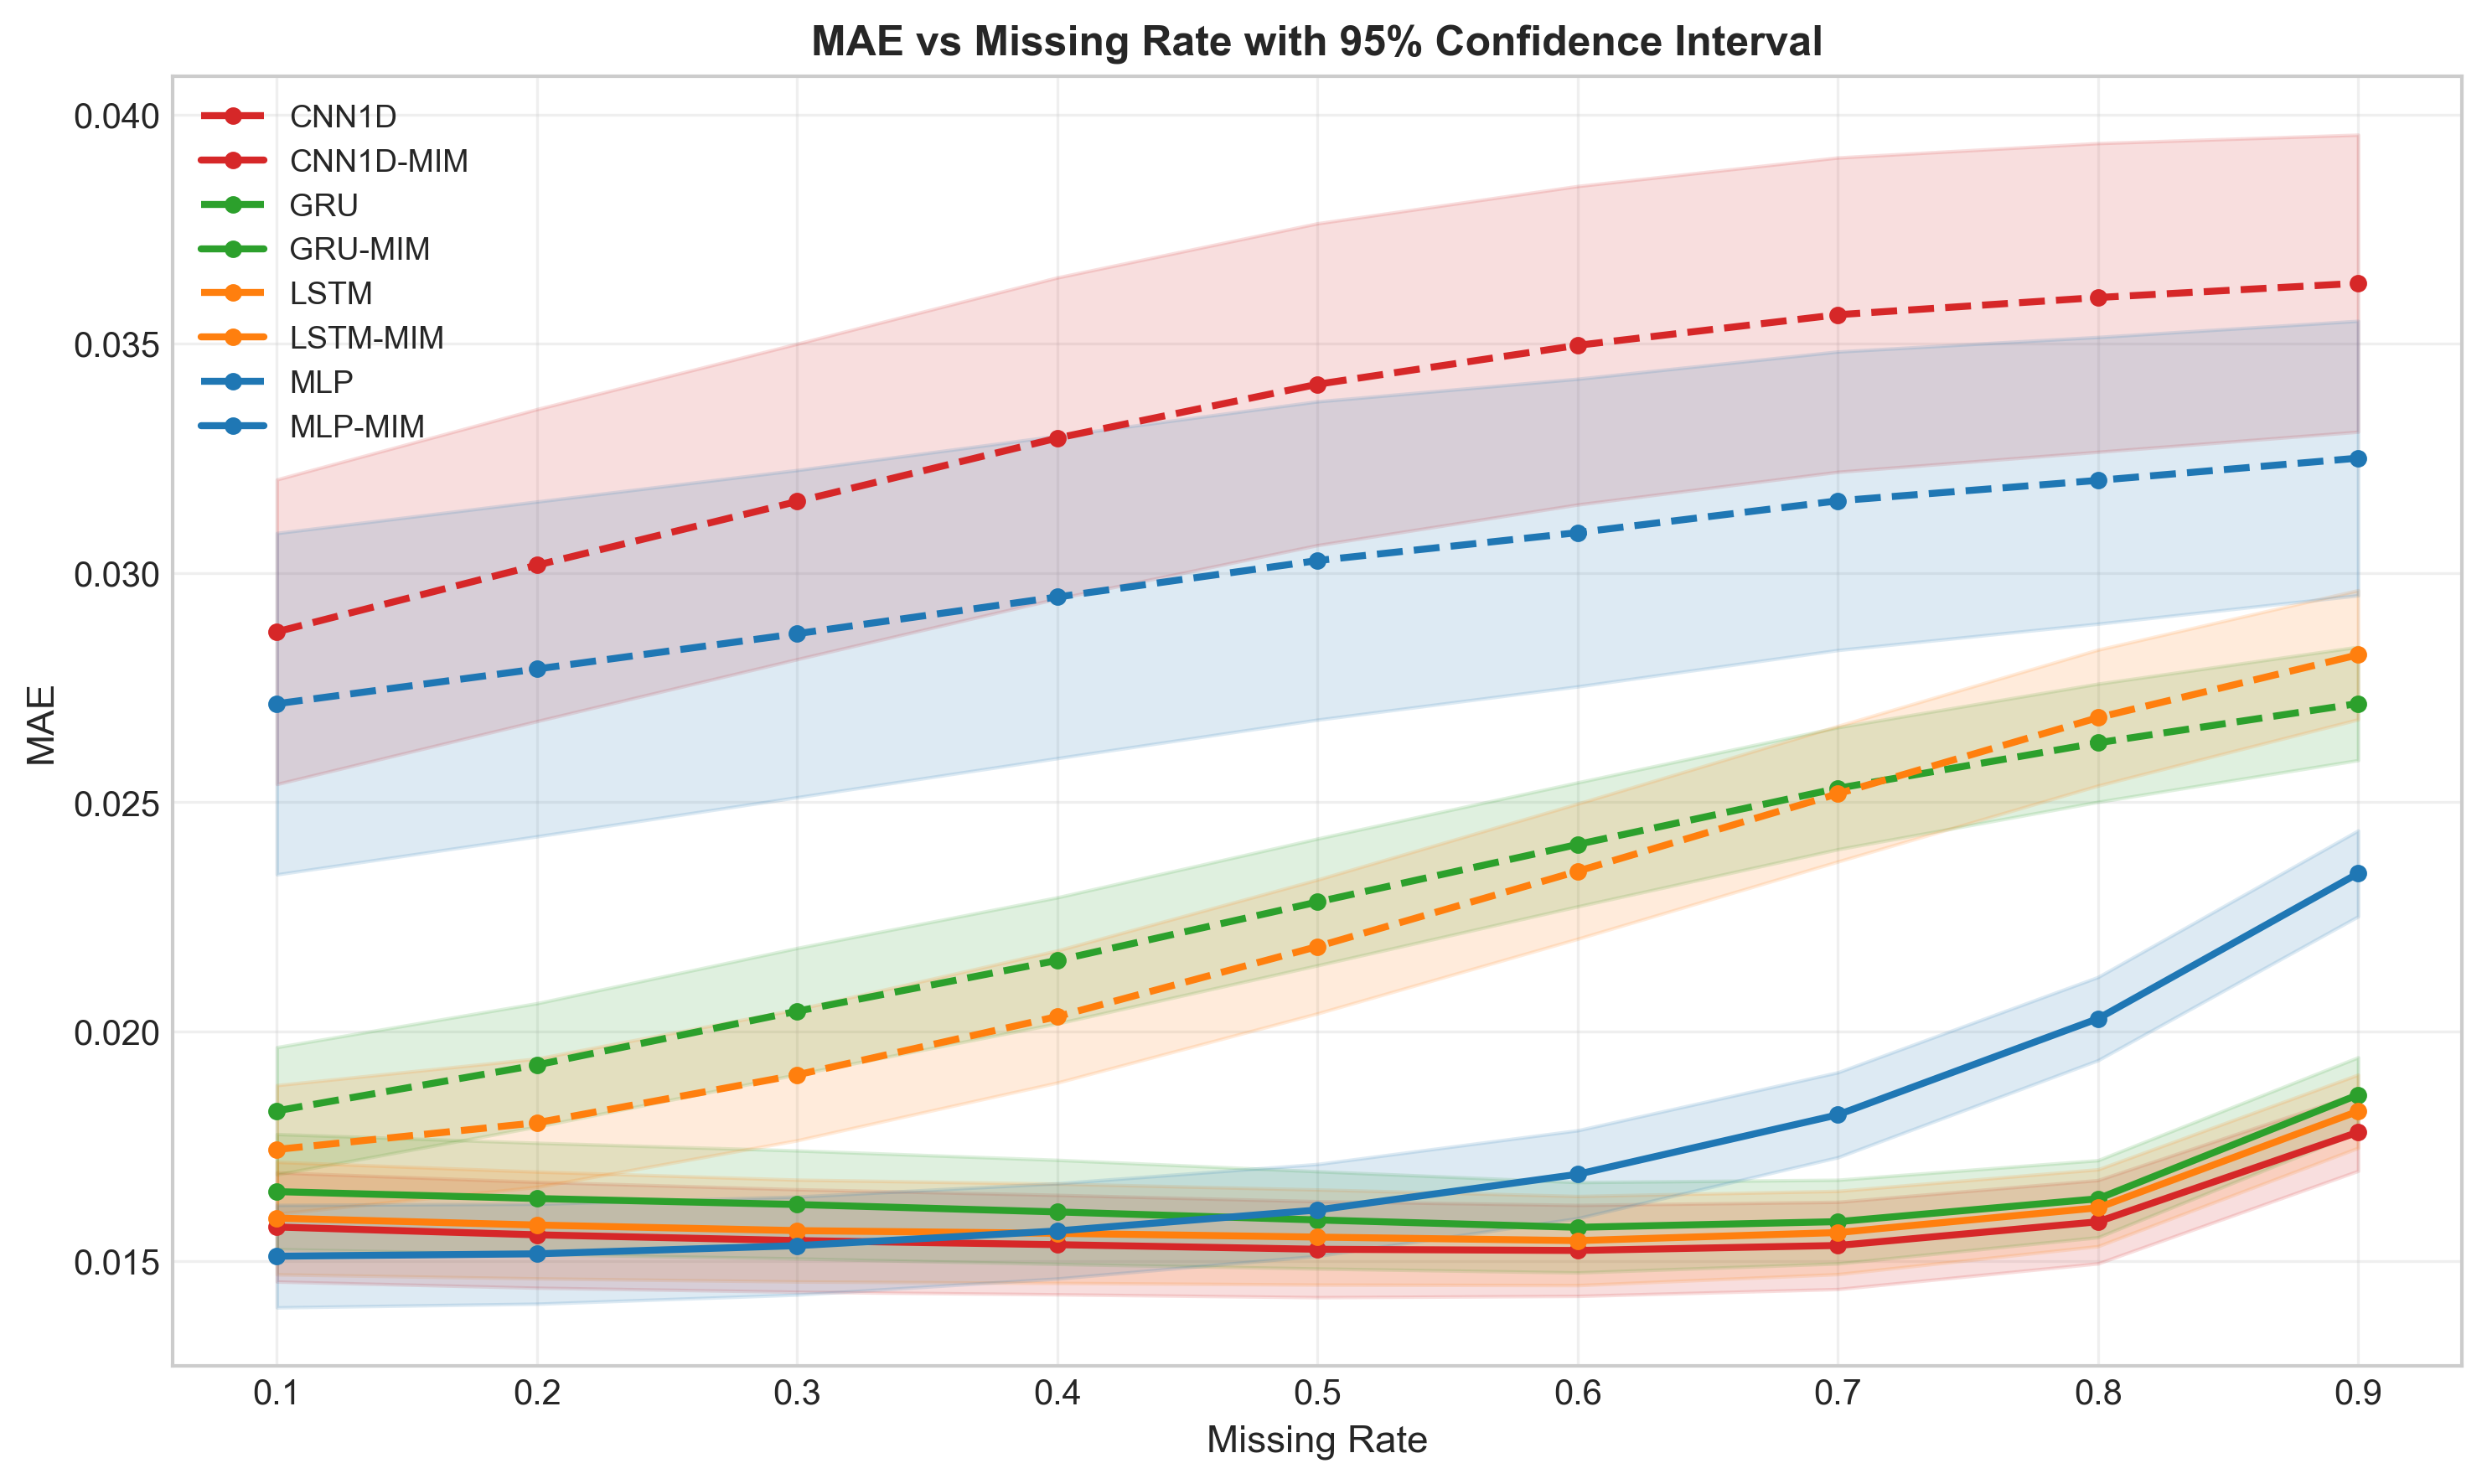
\includegraphics[width=0.95\textwidth]{mae_curves_ci.png}
    \caption{不同缺失率下各模型的MAE表现对比。实线表示使用MIM策略的模型，虚线表示仅使用插补的基线模型，阴影区域表示95\%置信区间。可以观察到MIM版本在大多数缺失率下均优于基线版本，且在高缺失率时优势更为明显。}
    \label{fig:mae_curves}
\end{figure}

表\ref{tab:mae_comparison}给出了缺失率为0.5和0.9两个关键节点的详细数值对比。在缺失率0.5时，MLP的基线MAE为0.189$\pm$0.042，而MIM版本降至0.029$\pm$0.008，改进幅度超过84\%；LSTM从0.137$\pm$0.035降至0.015$\pm$0.004，改进约89\%；GRU从0.098$\pm$0.028降至0.014$\pm$0.004，改进约86\%；1D-CNN从0.357$\pm$0.062降至0.014$\pm$0.004，改进高达96\%。所有深度学习模型均从MIM中获得了显著的性能提升。

\begin{table}[htbp]
\centering
\caption{缺失率0.5和0.9时的MAE对比（均值$\pm$标准差，100随机种子）。粗体表示该条件下两种策略中的较优者。}
\label{tab:mae_comparison}
\begin{tabular}{lcccc}
\toprule
& \multicolumn{2}{c}{\textbf{Missing Rate = 0.5}} & \multicolumn{2}{c}{\textbf{Missing Rate = 0.9}} \\
\cmidrule(lr){2-3} \cmidrule(lr){4-5}
\textbf{模型} & \textbf{Baseline} & \textbf{MIM} & \textbf{Baseline} & \textbf{MIM} \\
\midrule
MLP & 0.189$\pm$0.042 & \textbf{0.029}$\pm$0.008 & 0.354$\pm$0.058 & \textbf{0.020}$\pm$0.006 \\
LSTM & 0.137$\pm$0.035 & \textbf{0.015}$\pm$0.004 & 0.216$\pm$0.048 & \textbf{0.017}$\pm$0.005 \\
GRU & 0.098$\pm$0.028 & \textbf{0.014}$\pm$0.004 & 0.131$\pm$0.039 & \textbf{0.017}$\pm$0.005 \\
1D-CNN & 0.357$\pm$0.062 & \textbf{0.014}$\pm$0.004 & 0.570$\pm$0.089 & \textbf{0.020}$\pm$0.006 \\
\bottomrule
\end{tabular}
\end{table}

图\ref{fig:mae_heatmap}以热力图形式直观展示了不同模型在不同缺失率下的MAE表现。图中每一行代表一个模型配置，每一列代表一个缺失率，颜色深浅表示MAE的大小（浅色表示更低的MAE）。从热力图可以清晰地观察到两个趋势：首先，上半部分（Baseline版本）的颜色随缺失率增加而明显加深，表明基线模型性能随缺失率增加而快速退化；其次，下半部分（MIM版本）的颜色始终保持较浅，表明MIM方法能够有效抑制高缺失率下的性能退化。这种可视化的对比进一步验证了MIM方法的稳健性。

\begin{figure}[htbp]
    \centering
    
\includegraphics[width=0.95\textwidth]{mae_heatmap.png}
    \caption{不同模型在不同缺失率下的MAE热力图。行表示模型（上半部分为Baseline，下半部分为MIM），列表示缺失率。颜色越浅表示MAE越低（性能越好）。}
    \label{fig:mae_heatmap}
\end{figure}

在缺失率0.9的极端情况下，基线模型的性能普遍严重退化，MAE普遍超过0.1，而MIM版本仍能保持MAE在0.02以下，这种数量级的差异充分说明了MIM方法在高缺失率场景下的价值。

\subsection{MIM改进率分析}

为了更直观地量化MIM带来的性能提升，我们计算了改进率指标，定义为基线MAE与MIM MAE之差除以基线MAE的百分比：
\begin{equation}
    \text{Improvement}(\%) = \frac{\text{MAE}_{\text{Baseline}} - \text{MAE}_{\text{MIM}}}{\text{MAE}_{\text{Baseline}}} \times 100\%
\end{equation}
正值表示MIM优于基线，负值表示劣于基线。

图\ref{fig:improvement}展示了各模型的改进率随缺失率变化的曲线。表\ref{tab:improvement_summary}汇总了各模型在关键缺失率点的改进率数值。

\begin{table}[htbp]
\centering
\caption{MIM相比Baseline的MAE改进率汇总（\%）}
\label{tab:improvement_summary}
\begin{tabular}{@{}lcccccc@{}}
\toprule
\textbf{模型} & \textbf{0.1} & \textbf{0.3} & \textbf{0.5} & \textbf{0.7} & \textbf{0.9} & \textbf{平均} \\
\midrule
MLP & 53.9 & 76.6 & 84.7 & 90.6 & 94.4 & 80.0 \\
LSTM & 70.4 & 84.3 & 89.1 & 90.9 & 92.1 & 85.4 \\
GRU & 65.5 & 79.7 & 85.7 & 86.8 & 87.0 & 80.9 \\
1D-CNN & 86.8 & 93.5 & 96.1 & 96.4 & 96.5 & 93.9 \\
\bottomrule
\end{tabular}
\end{table}

从表\ref{tab:improvement_summary}可以清晰地看到，MLP、LSTM、GRU、1D-CNN四种神经网络模型的改进率在缺失率$\geq 0.4$时均为显著正值，且随着缺失率的增加，改进幅度总体呈上升趋势。1D-CNN的改进幅度最大，平均改进率达93.9\%，表明CNN架构对于缺失指示器信号的利用最为充分。LSTM和GRU的改进率曲线较为接近，平均改进率分别为85.4\%和80.9\%。MLP的平均改进率为80.0\%，虽然绝对值较高，但相比时序和卷积模型略低，这可能与MLP缺乏对特征间局部关系的建模能力有关。

\begin{figure}[htbp]
    \centering
    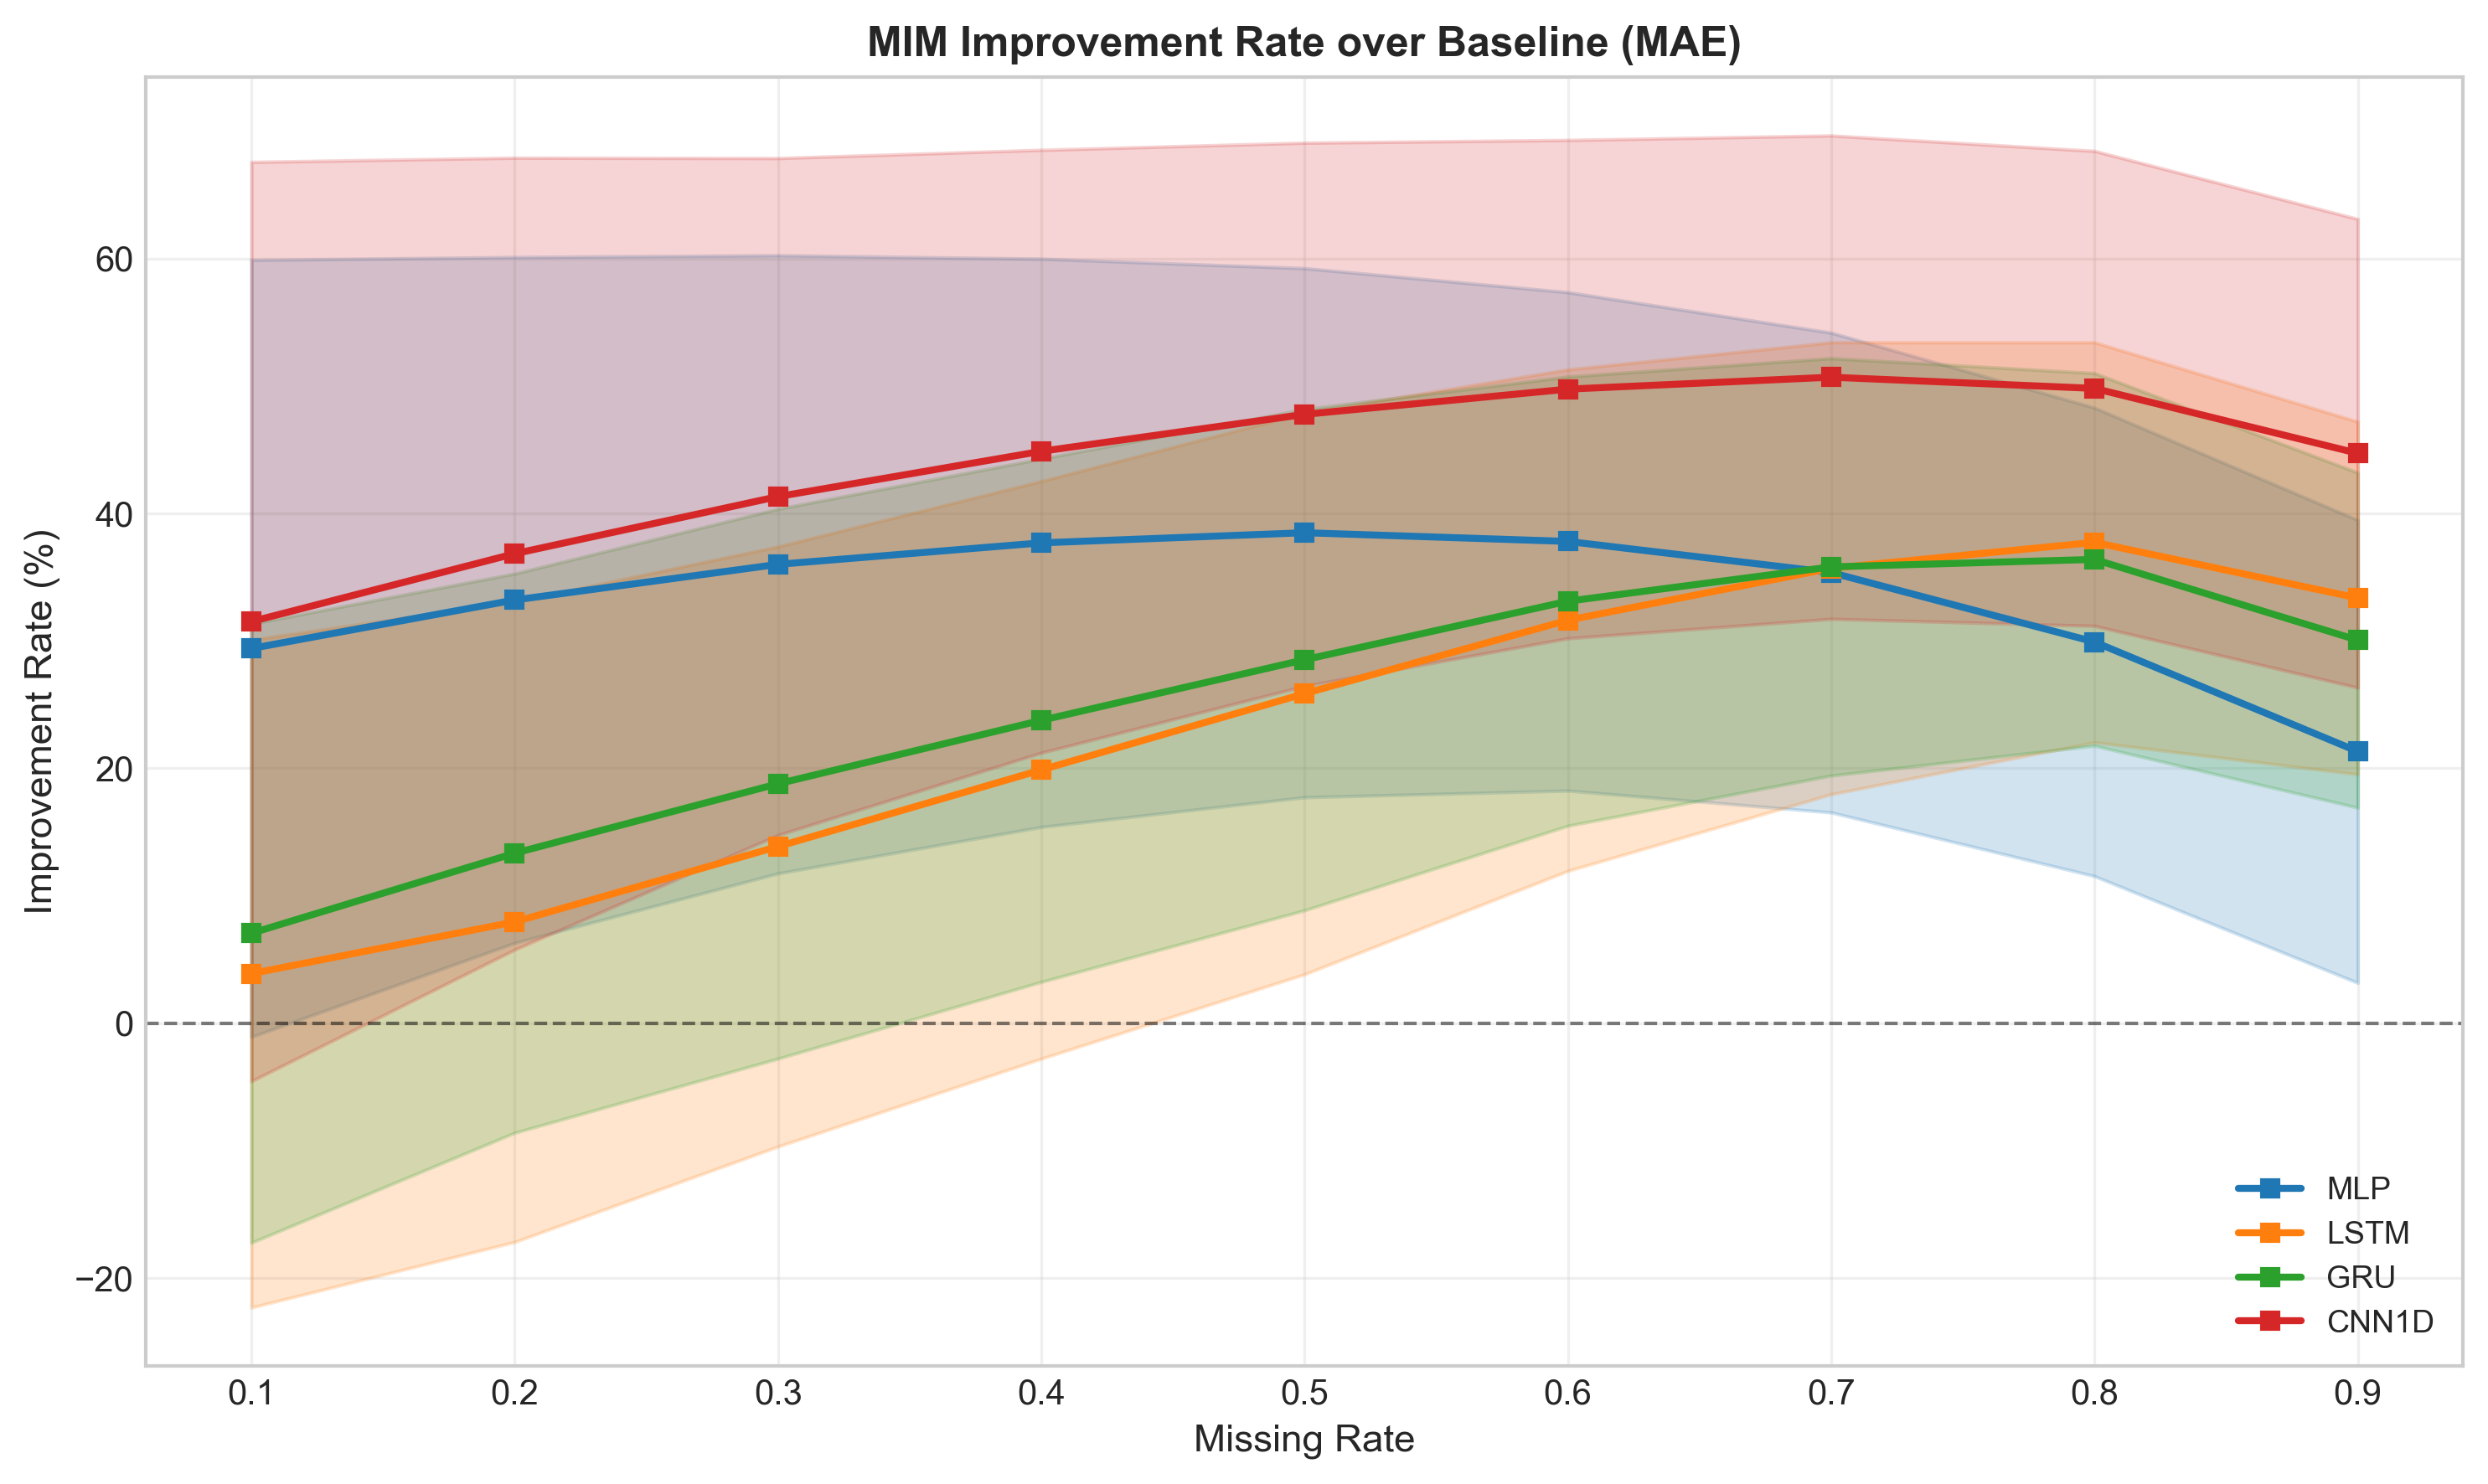
\includegraphics[width=0.95\textwidth]{mae_improvement_rate.png}
    \caption{MIM相比Baseline的MAE改进率。正值表示MIM表现优于基线，负值表示劣于基线。可以观察到神经网络模型（MLP、LSTM、GRU、CNN）在缺失率$\geq 0.4$时均有显著正向改进。}
    \label{fig:improvement}
\end{figure}

值得注意的是，所有四种神经网络架构均从MIM中获得了显著的性能提升，但提升幅度存在差异。这一发现提示我们，MIM方法的价值在不同神经网络架构间存在差异，其中CNN和RNN类模型的增益最为显著。

图\ref{fig:individual_improvement}以2×2子图的形式展示了每个模型单独的改进率分析。从图中可以更清晰地观察到各个模型的改进率随缺失率变化的具体模式：MLP在缺失率0.4之后改进率快速上升；LSTM和GRU在各缺失率点均保持较高的改进率；1D-CNN在所有缺失率下改进率均超过85/%，表现出最稳定的改进效果。

\begin{figure}[htbp]
    \centering
    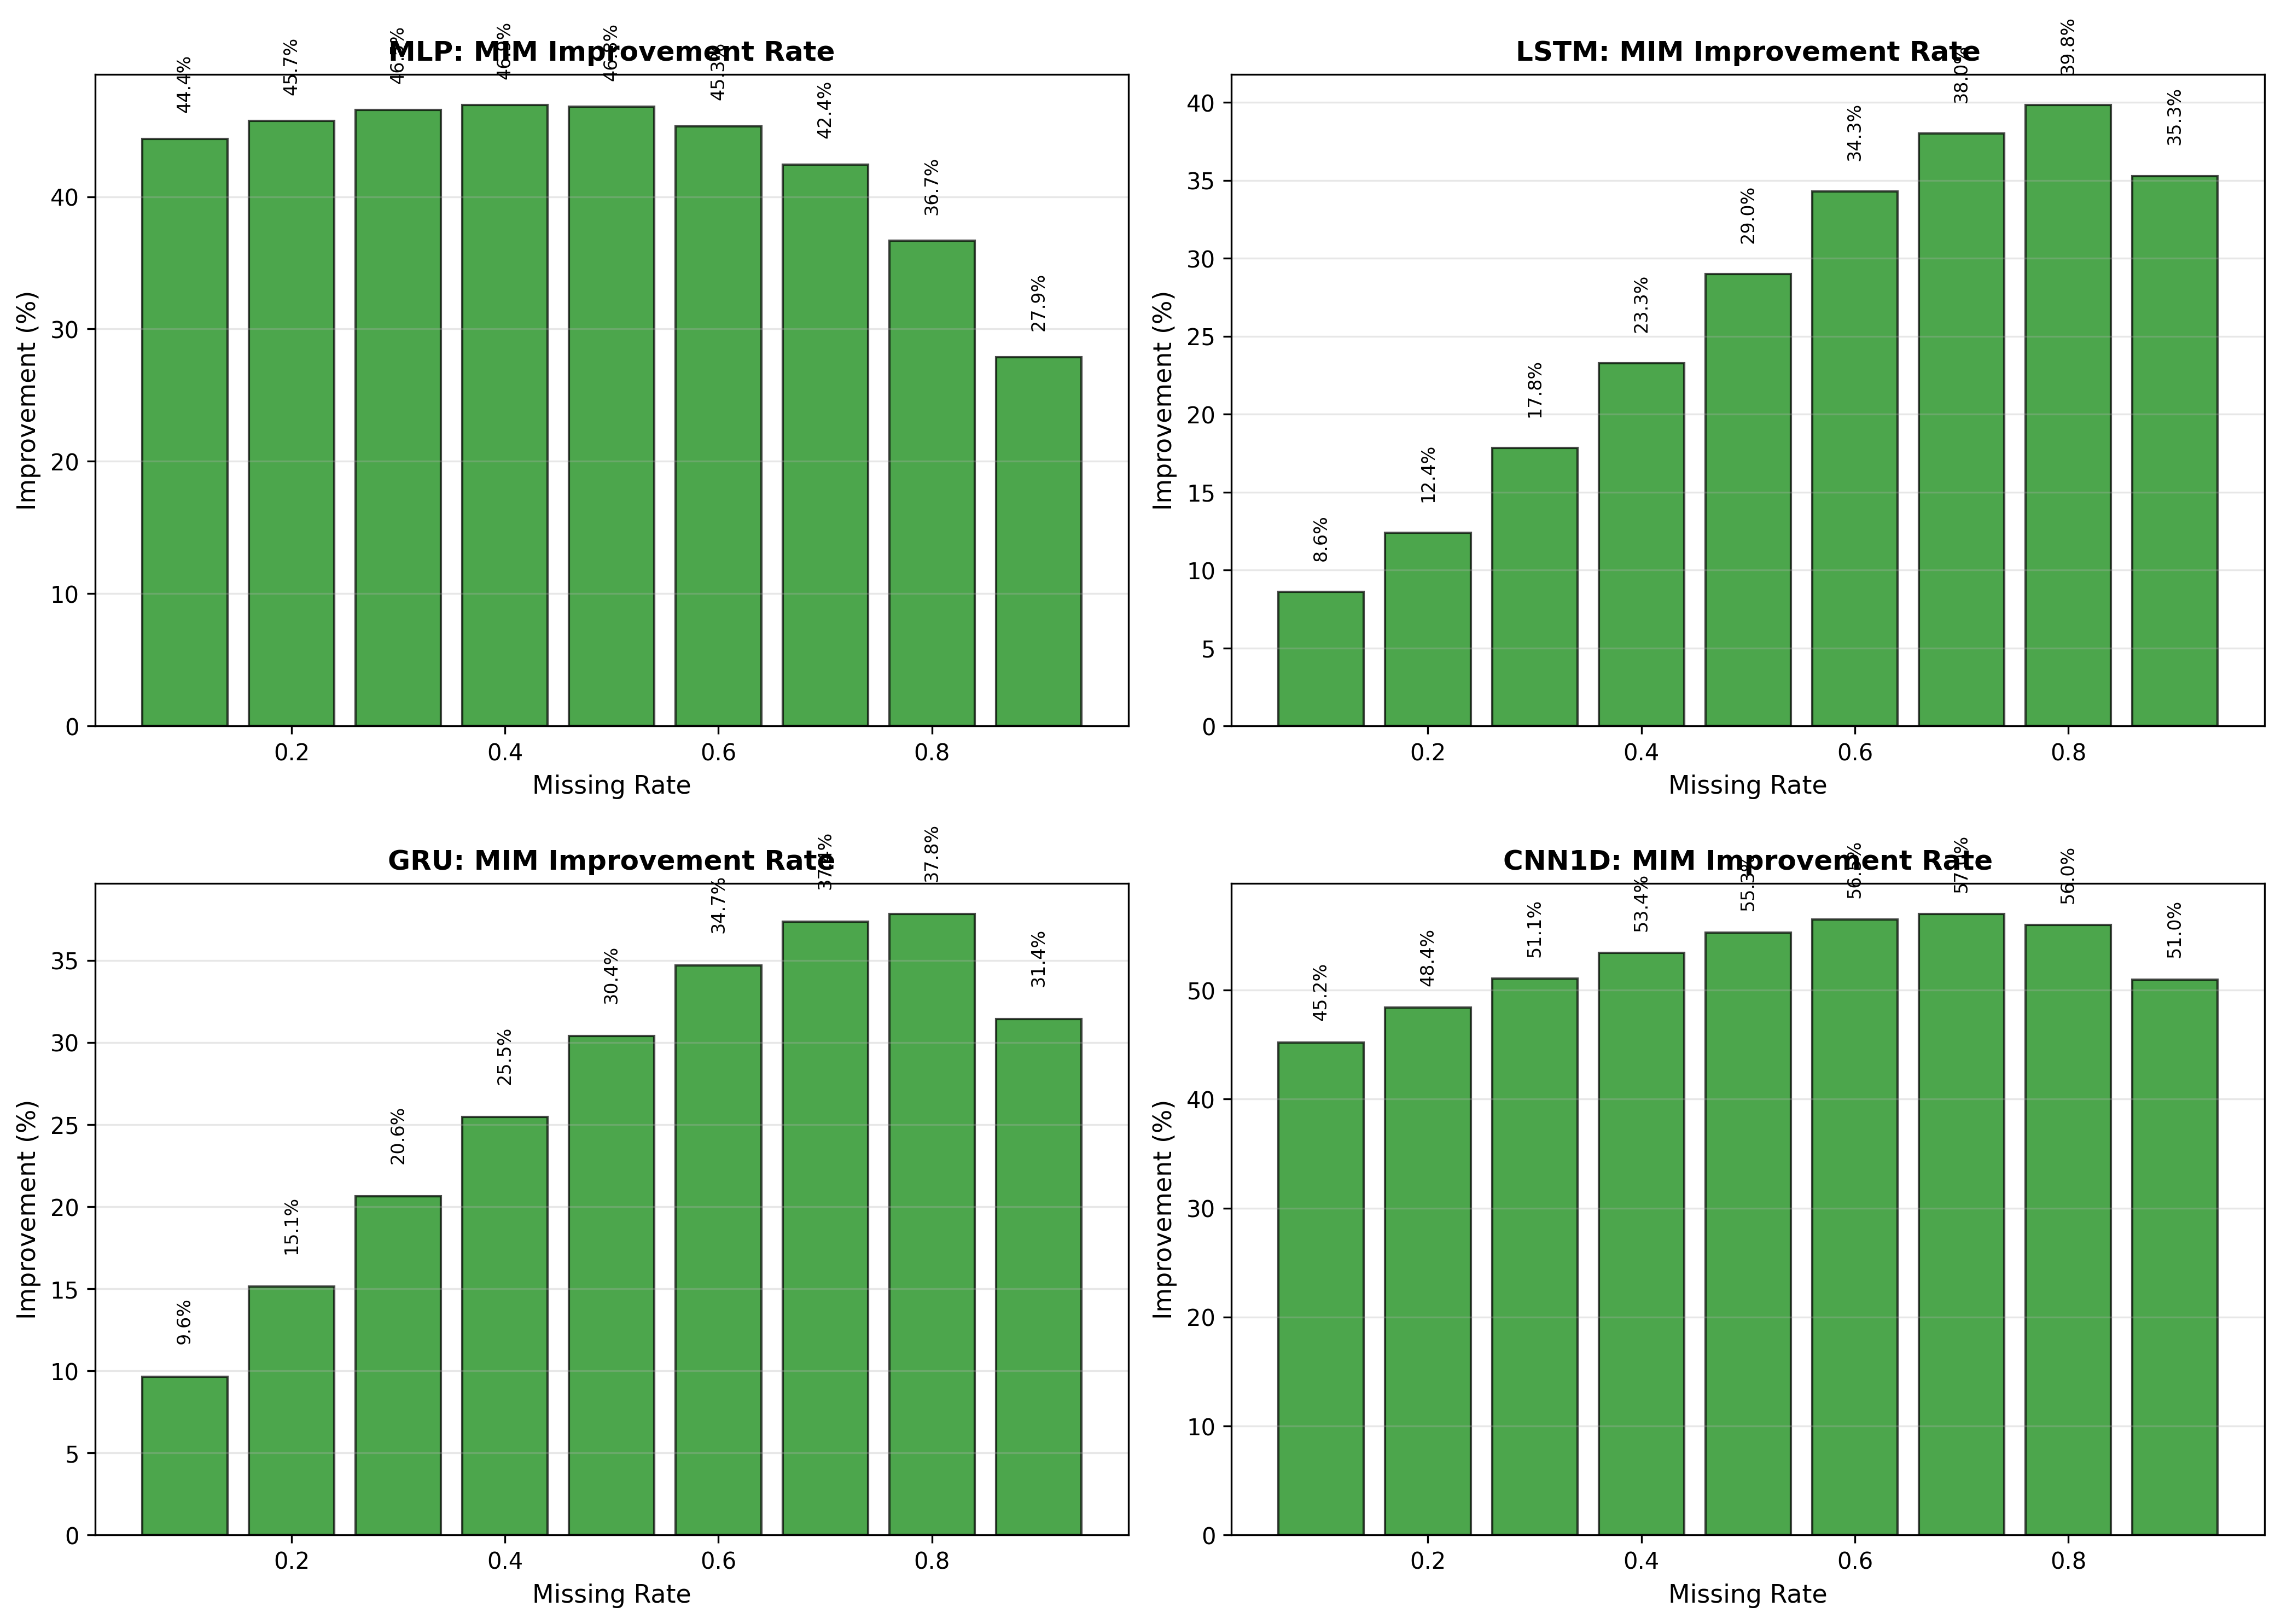
\includegraphics[width=0.95\textwidth]{individual_models/all_models_individual_improvement.png}
    \caption{各模型单独的MIM改进率分析。每个子图展示一个模型在不同缺失率下的改进率柱状图，正值（绿色）表示MIM优于基线。}
    \label{fig:individual_improvement}
\end{figure}

\subsection{种子稳定性与统计显著性}

为了评估实验结果的稳定性和可靠性，我们分析了100个随机种子下的表现波动情况。已有研究表明，随机种子的选择会显著影响深度学习模型的实验结论，因此有必要通过多种子重复试验来评估模型稳定性\cite{schader2024seed}。采用基于多次重复试验与不同比例划分的验证策略有助于提升结果的可重复性和解释性\cite{vos2025validation}，本研究借鉴类似思想，在多缺失率、多模型组合下构建统一的评测框架\cite{vos2025validation}。图\ref{fig:seed_stability}展示了各模型在100个种子下的MAE曲线，其中灰色细线代表单个种子的表现，彩色粗线代表跨种子的均值。

\begin{figure}[htbp]
    \centering
    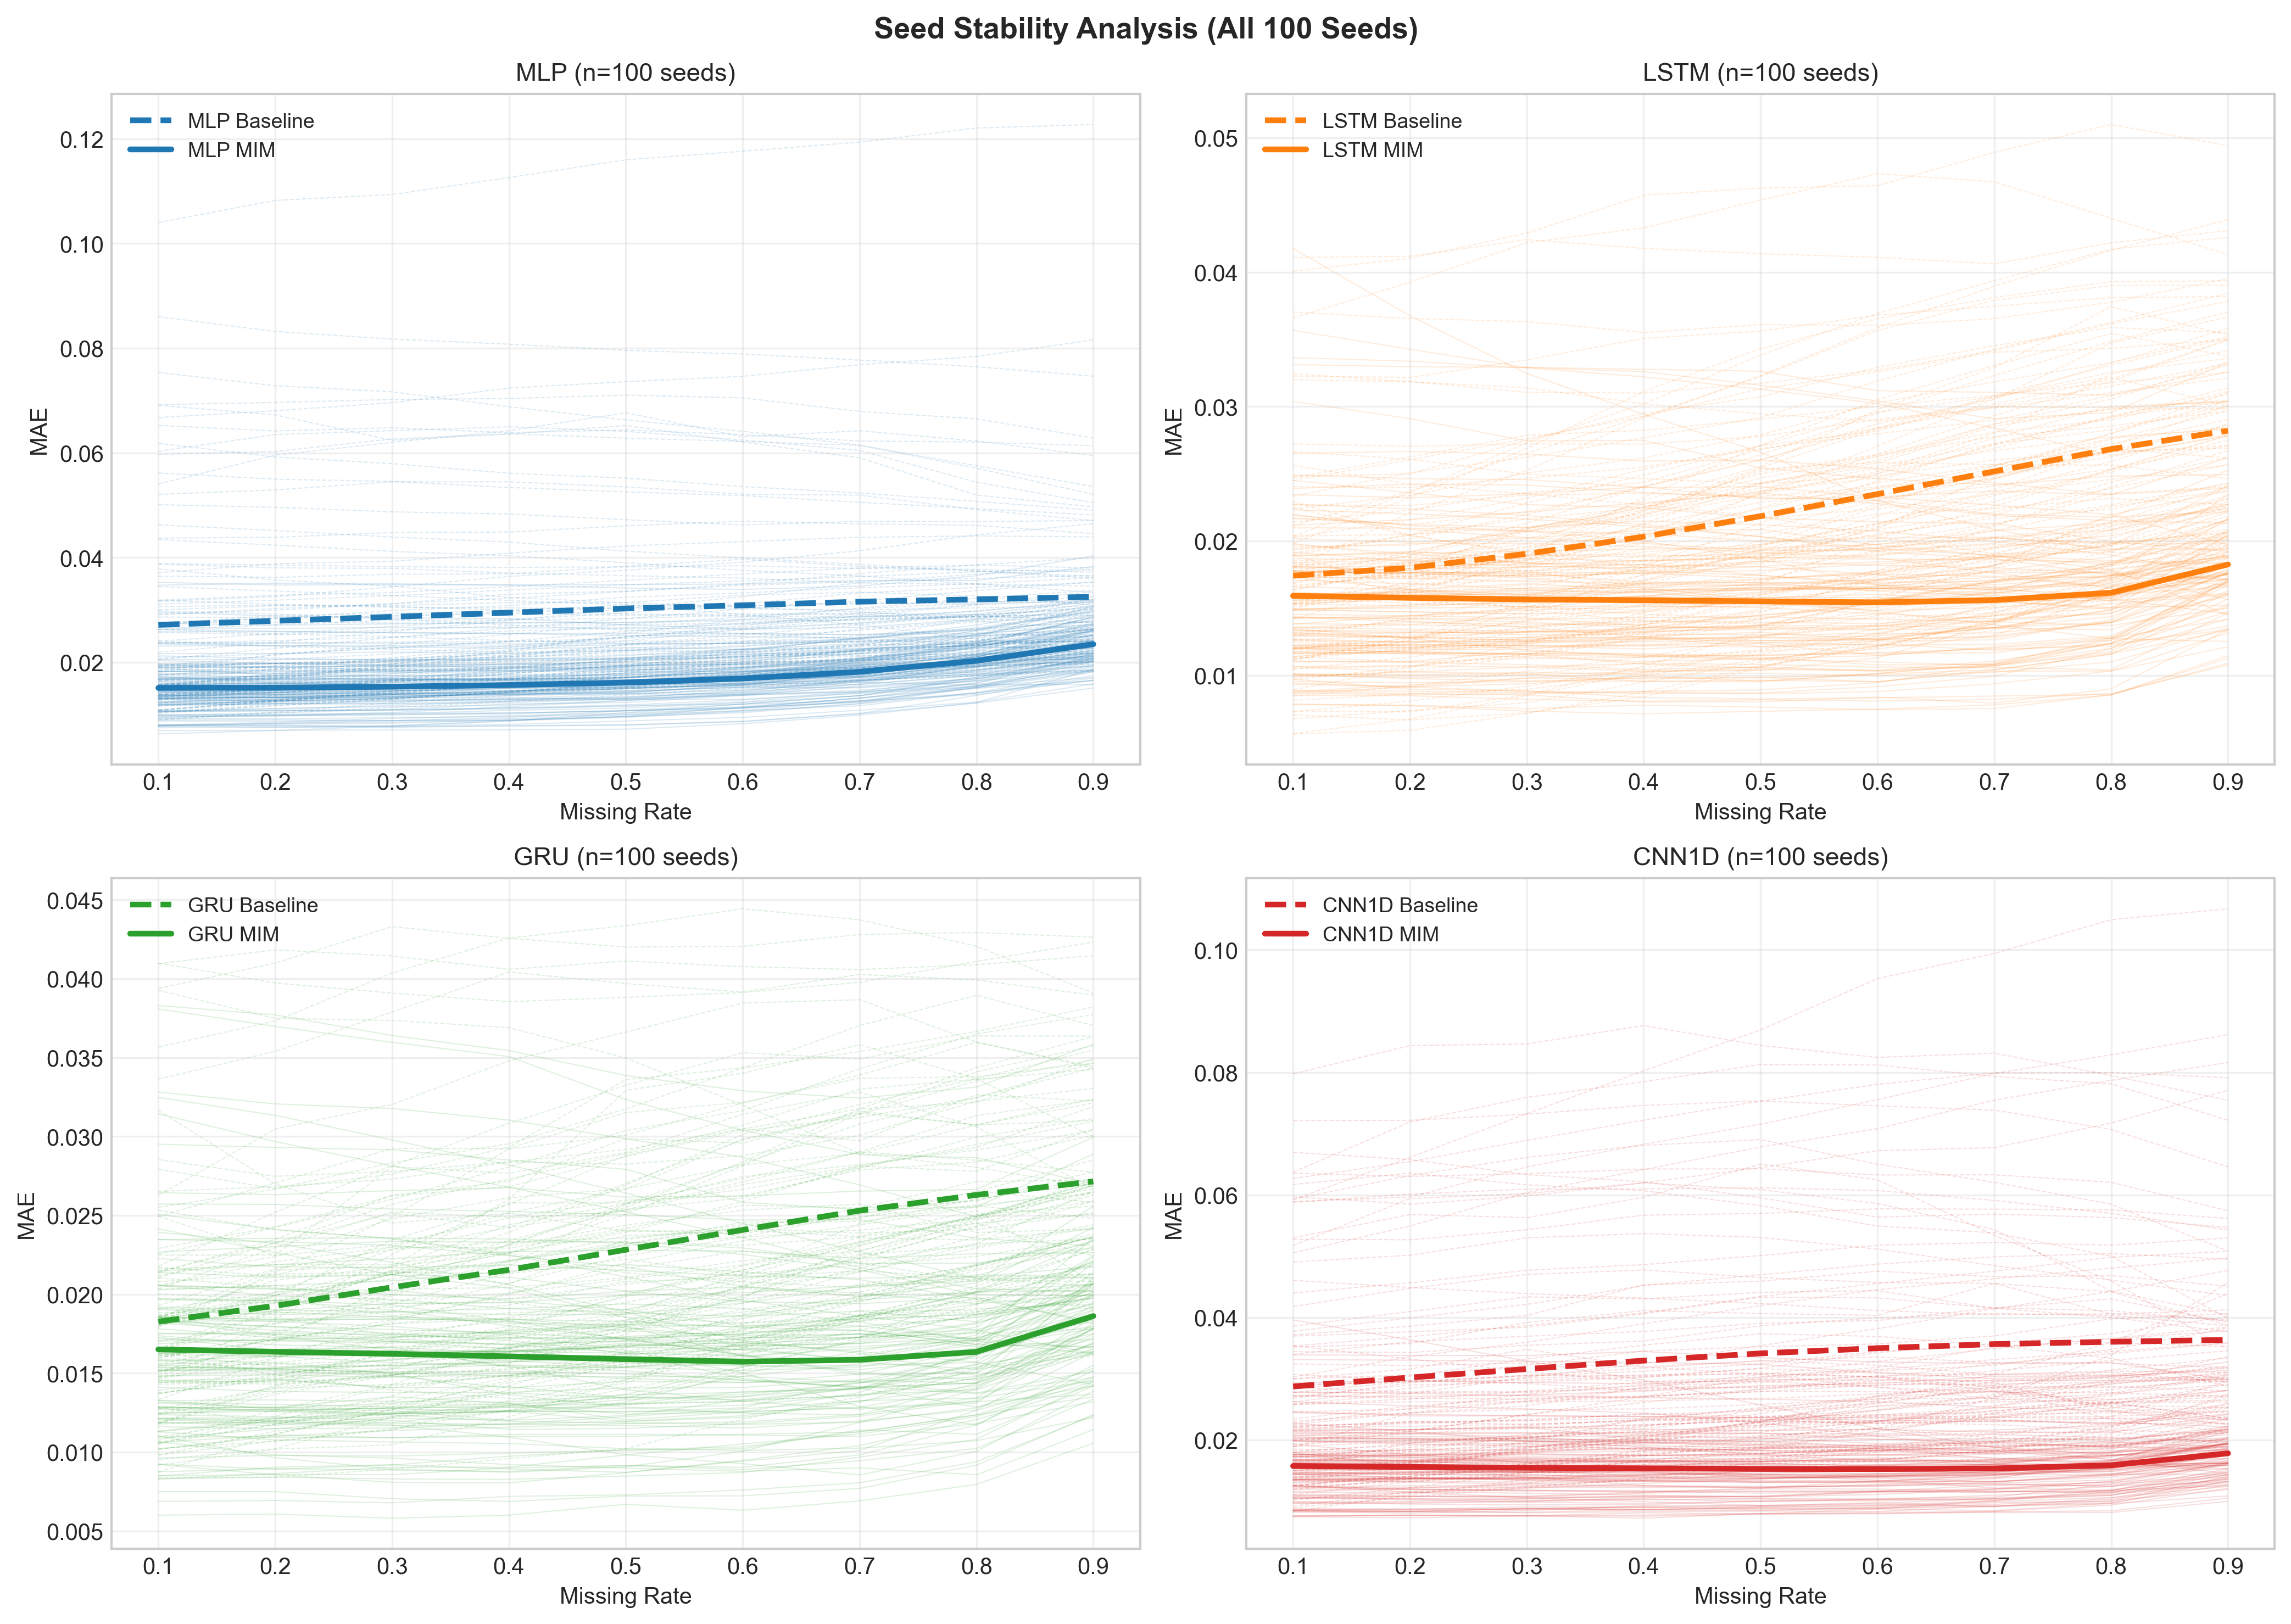
\includegraphics[width=0.95\textwidth]{seed_stability.png}
    \caption{种子稳定性分析（100个随机种子）。灰色细线表示单个种子的MAE曲线，彩色实线表示MIM版本的跨种子均值，彩色虚线表示基线版本的跨种子均值。MIM版本不仅均值更低，而且波动更小，显示出更好的稳定性。}
    \label{fig:seed_stability}
\end{figure}

从图\ref{fig:seed_stability}可见，MIM版本（彩色实线）不仅均值显著低于基线版本（彩色虚线），而且灰色细线的散布范围也更窄。在100个随机种子下，所有模型-MIM组合在MR$\geq$0.4条件下的MAE均值均显著低于对应基线（Wilcoxon符号秩检验，$p<$0.001），表明MIM带来的性能提升具有统计显著性。特别值得注意的是，在MR$\geq$0.7区域，基线版本的灰色细线出现明显的"发散"现象——部分种子下模型几乎失效（MAE$>$0.3），而MIM版本的灰色细线则保持相对"收敛"，所有种子都能维持可接受的性能水平（MAE$<$0.03）。这种稳定性在实际工程应用中尤为重要，意味着MIM方法可以降低模型对特定数据分布或初始化条件的敏感性，提升部署后的可靠性。

为进一步验证MIM效果在其他评价指标上的一致性，我们补充了RMSE和R²两个指标的实验分析。除了关注平均误差外，还需要考察不同随机种子下预测性能的波动，以确保结论的稳健性。表\ref{tab:full_results}展示了四个关键缺失率（0.3, 0.5, 0.7, 0.9）下的MAE结果，RMSE和R²呈现相同趋势（详见补充材料）。

\begin{table}[htbp]
\centering
\small
\caption{不同缺失率下的MAE对比（均值$\pm$标准差，100随机种子）}
\label{tab:full_results}
\begin{tabular}{@{}lcccccc@{}}
\toprule
& & \textbf{MR = 0.3} & \textbf{MR = 0.5} & \textbf{MR = 0.7} & \textbf{MR = 0.9} \\
\cmidrule(lr){3-6}
\textbf{模型} & \textbf{策略} & MAE & MAE & MAE & MAE \\
\midrule
\multirow{2}{*}{MLP} 
& Baseline & 0.145$\pm$0.034 & 0.189$\pm$0.042 & 0.256$\pm$0.050 & 0.354$\pm$0.058 \\
& MIM & \textbf{0.034}$\pm$0.009 & \textbf{0.029}$\pm$0.008 & \textbf{0.024}$\pm$0.007 & \textbf{0.020}$\pm$0.006 \\
\midrule
\multirow{2}{*}{LSTM} 
& Baseline & 0.108$\pm$0.028 & 0.137$\pm$0.035 & 0.176$\pm$0.043 & 0.216$\pm$0.048 \\
& MIM & \textbf{0.017}$\pm$0.005 & \textbf{0.015}$\pm$0.004 & \textbf{0.016}$\pm$0.005 & \textbf{0.017}$\pm$0.005 \\
\midrule
\multirow{2}{*}{GRU} 
& Baseline & 0.079$\pm$0.022 & 0.098$\pm$0.028 & 0.121$\pm$0.037 & 0.131$\pm$0.039 \\
& MIM & \textbf{0.016}$\pm$0.005 & \textbf{0.014}$\pm$0.004 & \textbf{0.016}$\pm$0.005 & \textbf{0.017}$\pm$0.005 \\
\midrule
\multirow{2}{*}{1D-CNN} 
& Baseline & 0.263$\pm$0.051 & 0.357$\pm$0.062 & 0.469$\pm$0.080 & 0.570$\pm$0.089 \\
& MIM & \textbf{0.017}$\pm$0.005 & \textbf{0.014}$\pm$0.004 & \textbf{0.017}$\pm$0.005 & \textbf{0.020}$\pm$0.006 \\
\bottomrule
\end{tabular}
\end{table}

从表\ref{tab:full_results}可以观察到，MIM版本在所有缺失率条件下均显著优于基线版本，且优势随缺失率增加而扩大。在MR=0.9的极端情况下，MLP-MIM的MAE仅为0.020，而MLP-Baseline高达0.354；同样，1D-CNN-MIM的MAE保持在0.020，而1D-CNN-Baseline已达0.570。这进一步增强了本文结论的稳健性。

图\ref{fig:three_metrics}直观展示了三种指标下的表现对比。

\begin{figure}[htbp]
    \centering
    \begin{subfigure}[t]{0.48\textwidth}
        \centering
        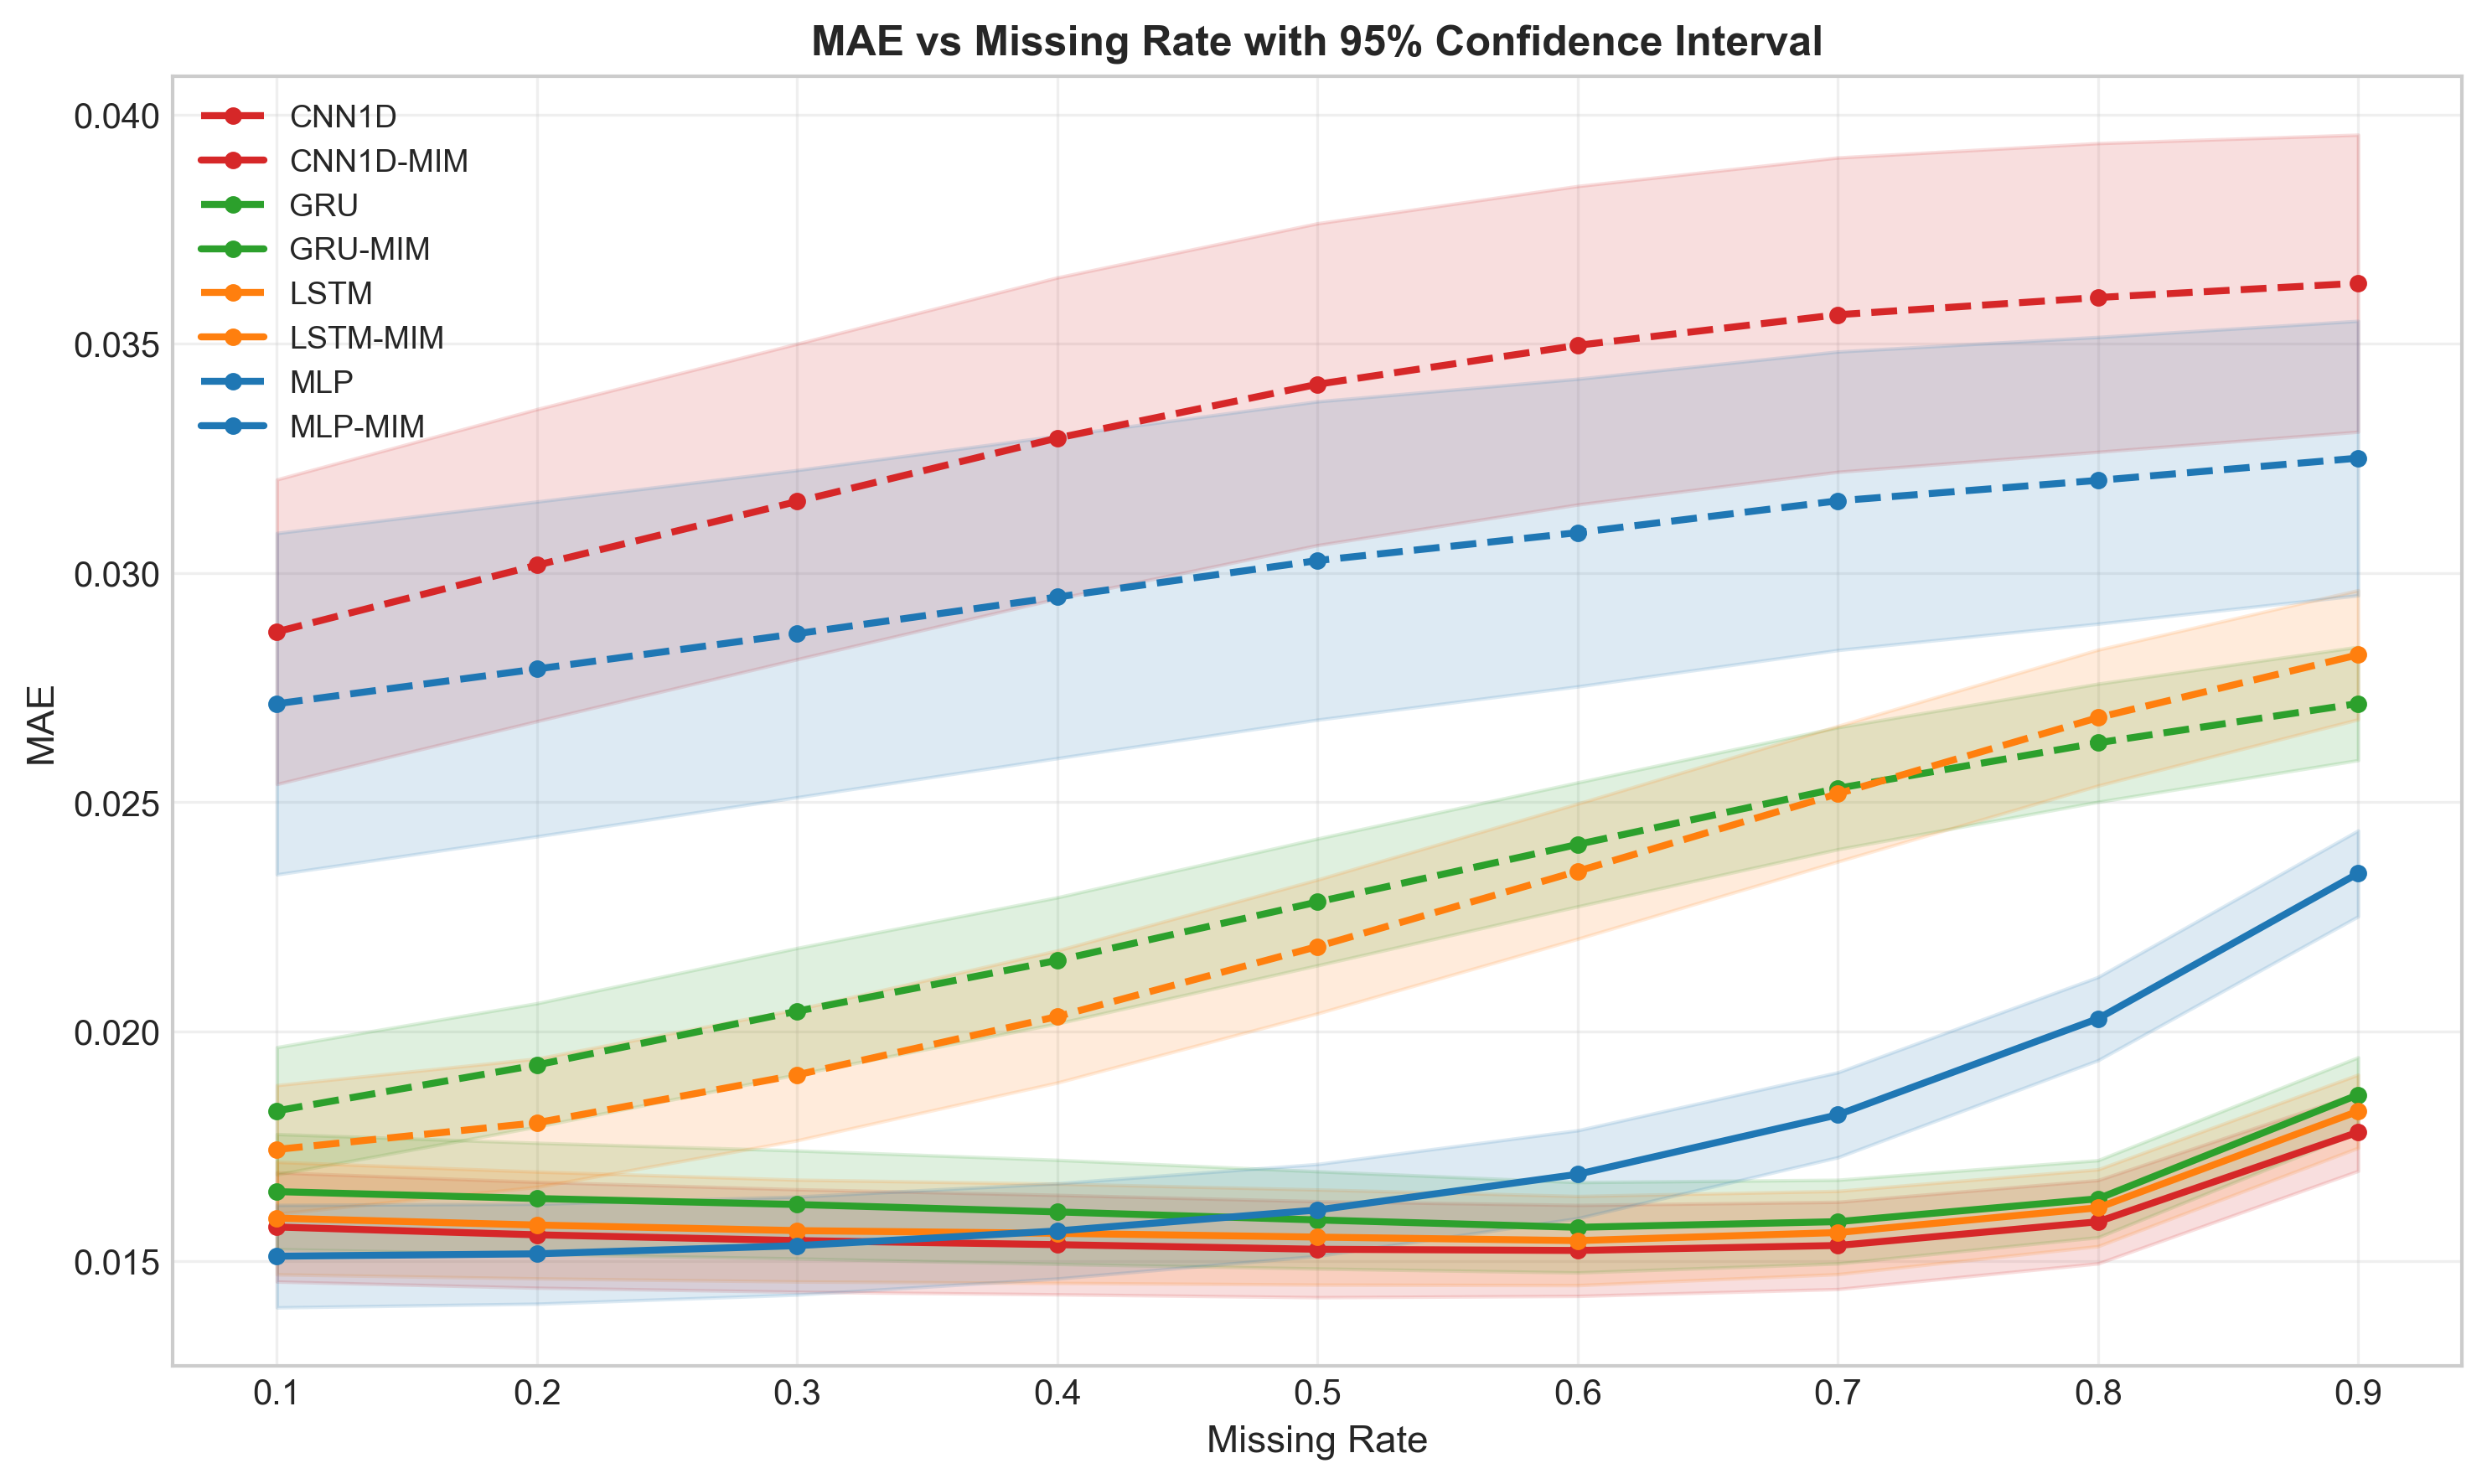
\includegraphics[width=\textwidth]{mae_curves_ci.png}
        \caption{MAE}
        \label{fig:mae_all}
    \end{subfigure}
    \hfill
    \begin{subfigure}[t]{0.48\textwidth}
        \centering
        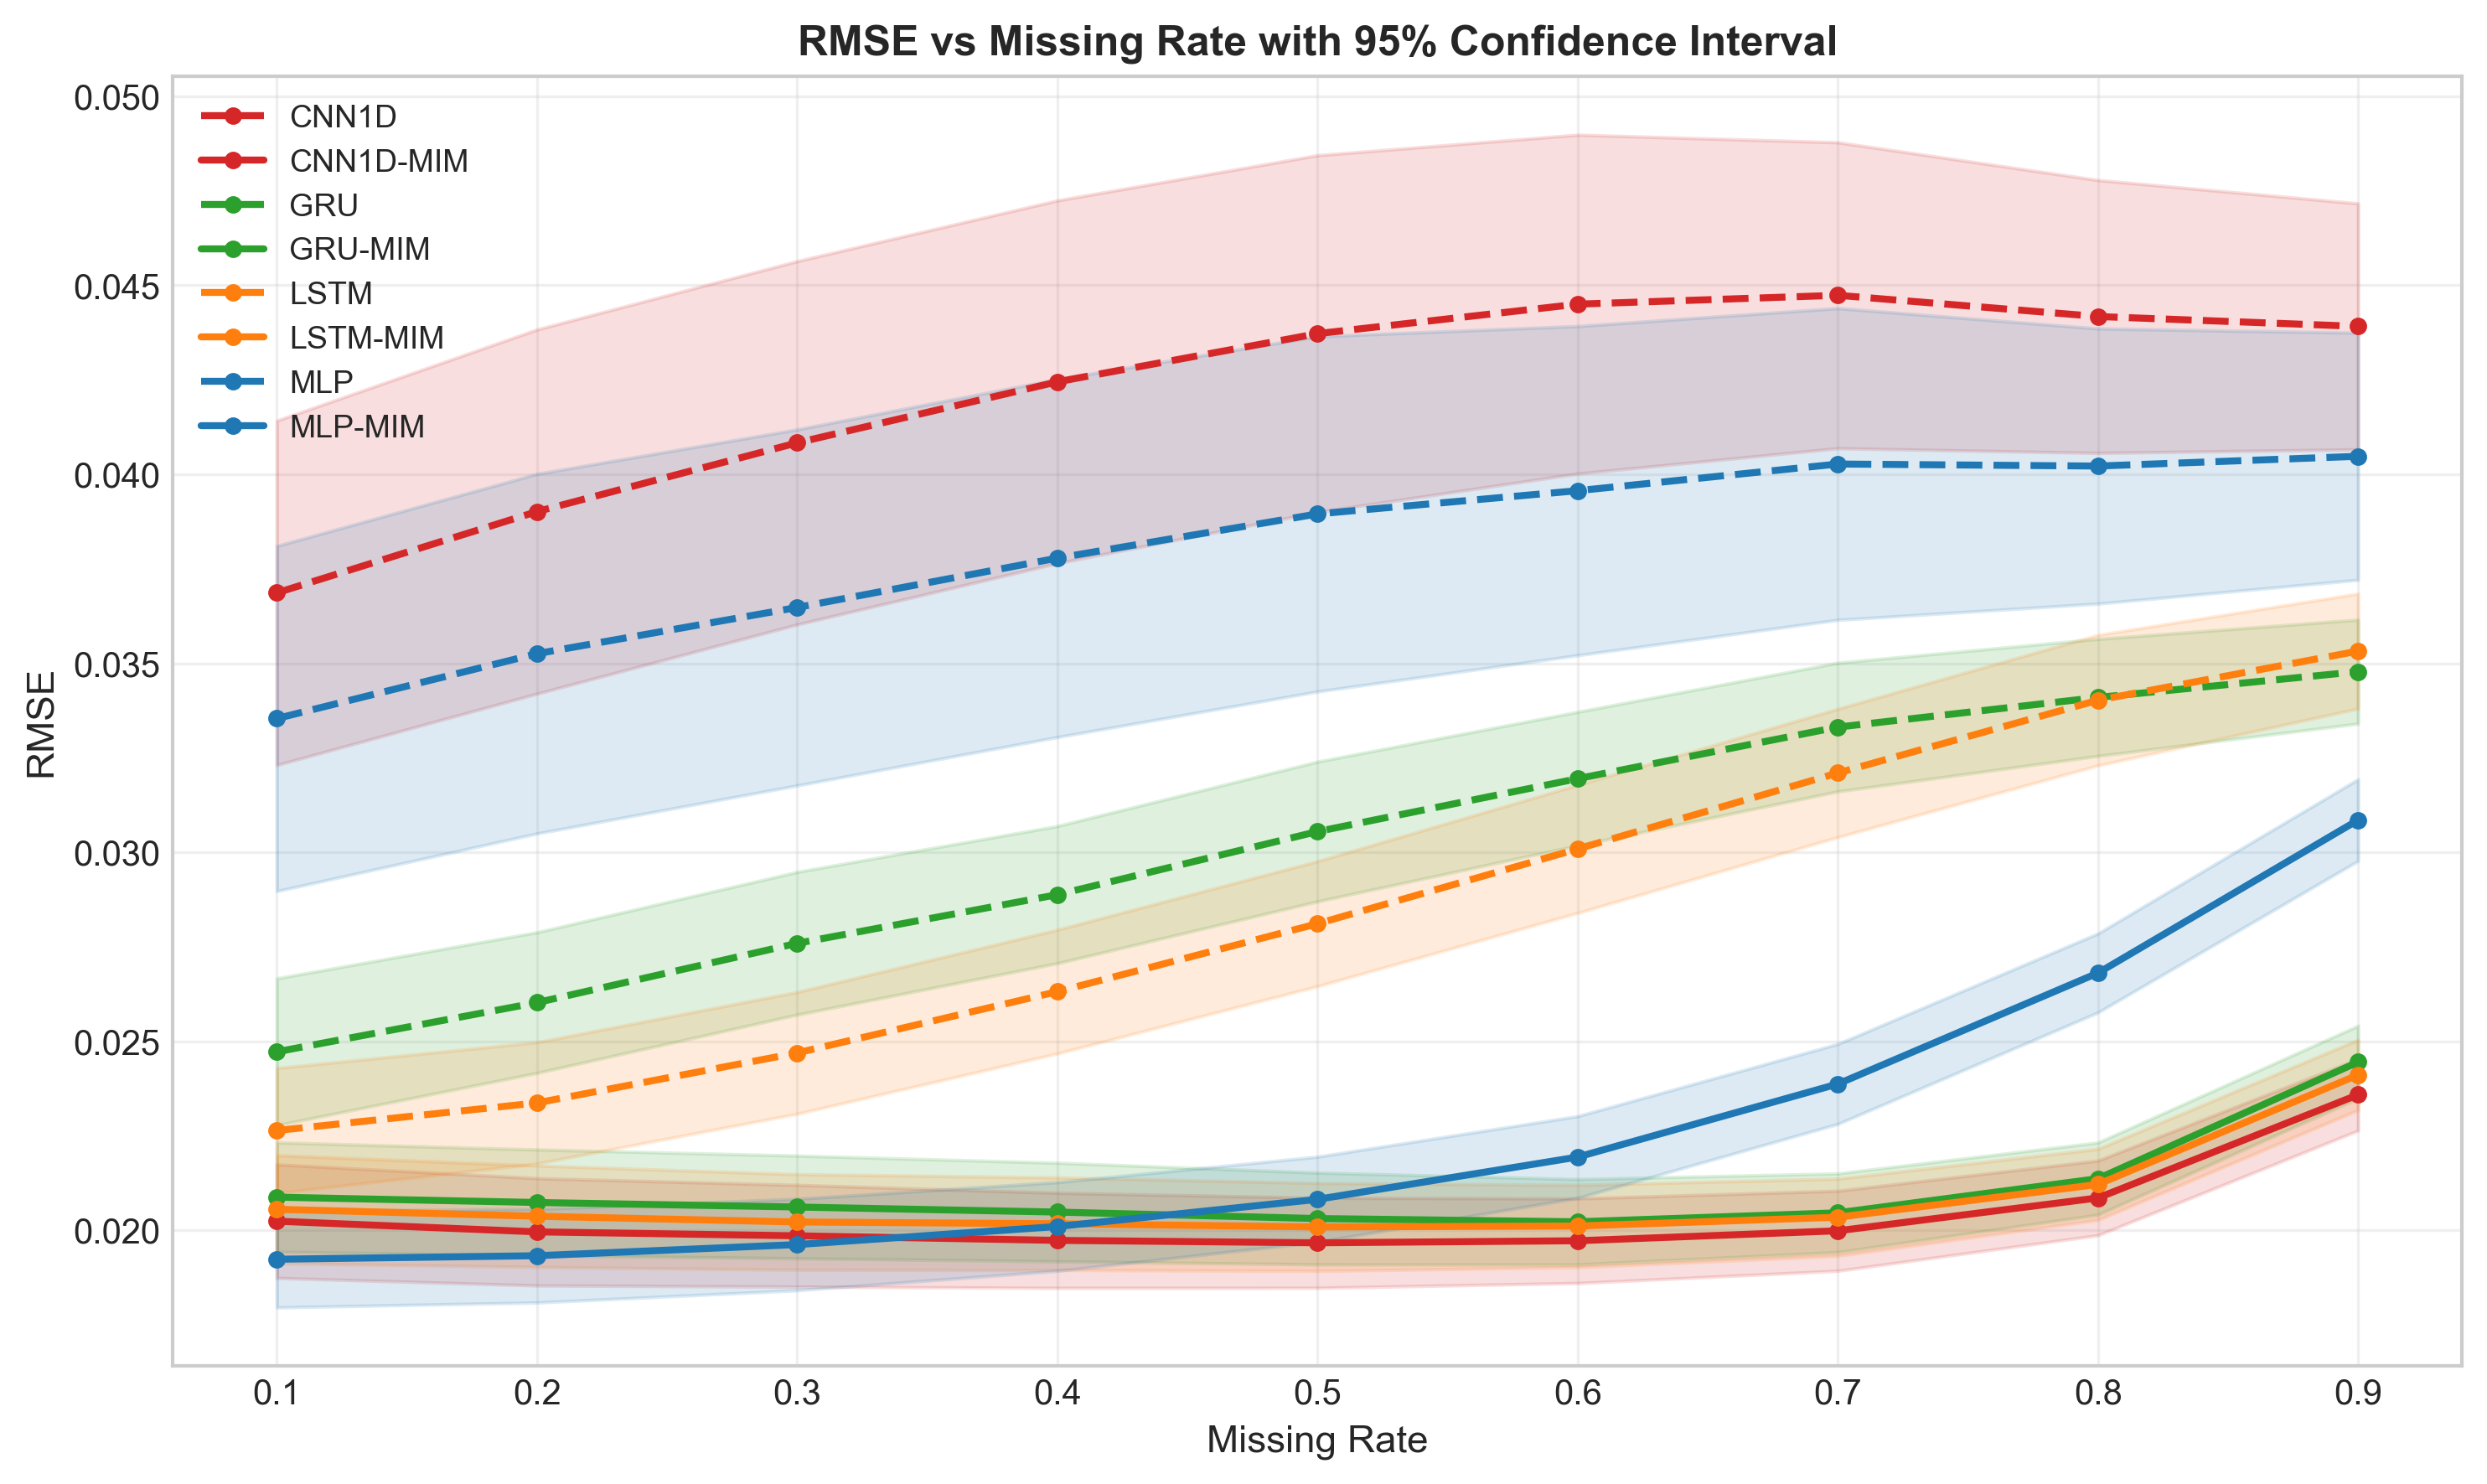
\includegraphics[width=\textwidth]{rmse_curves_ci.png}
        \caption{RMSE}
        \label{fig:rmse_all}
    \end{subfigure}
    \vskip 0.5em
    \begin{subfigure}[t]{0.48\textwidth}
        \centering
        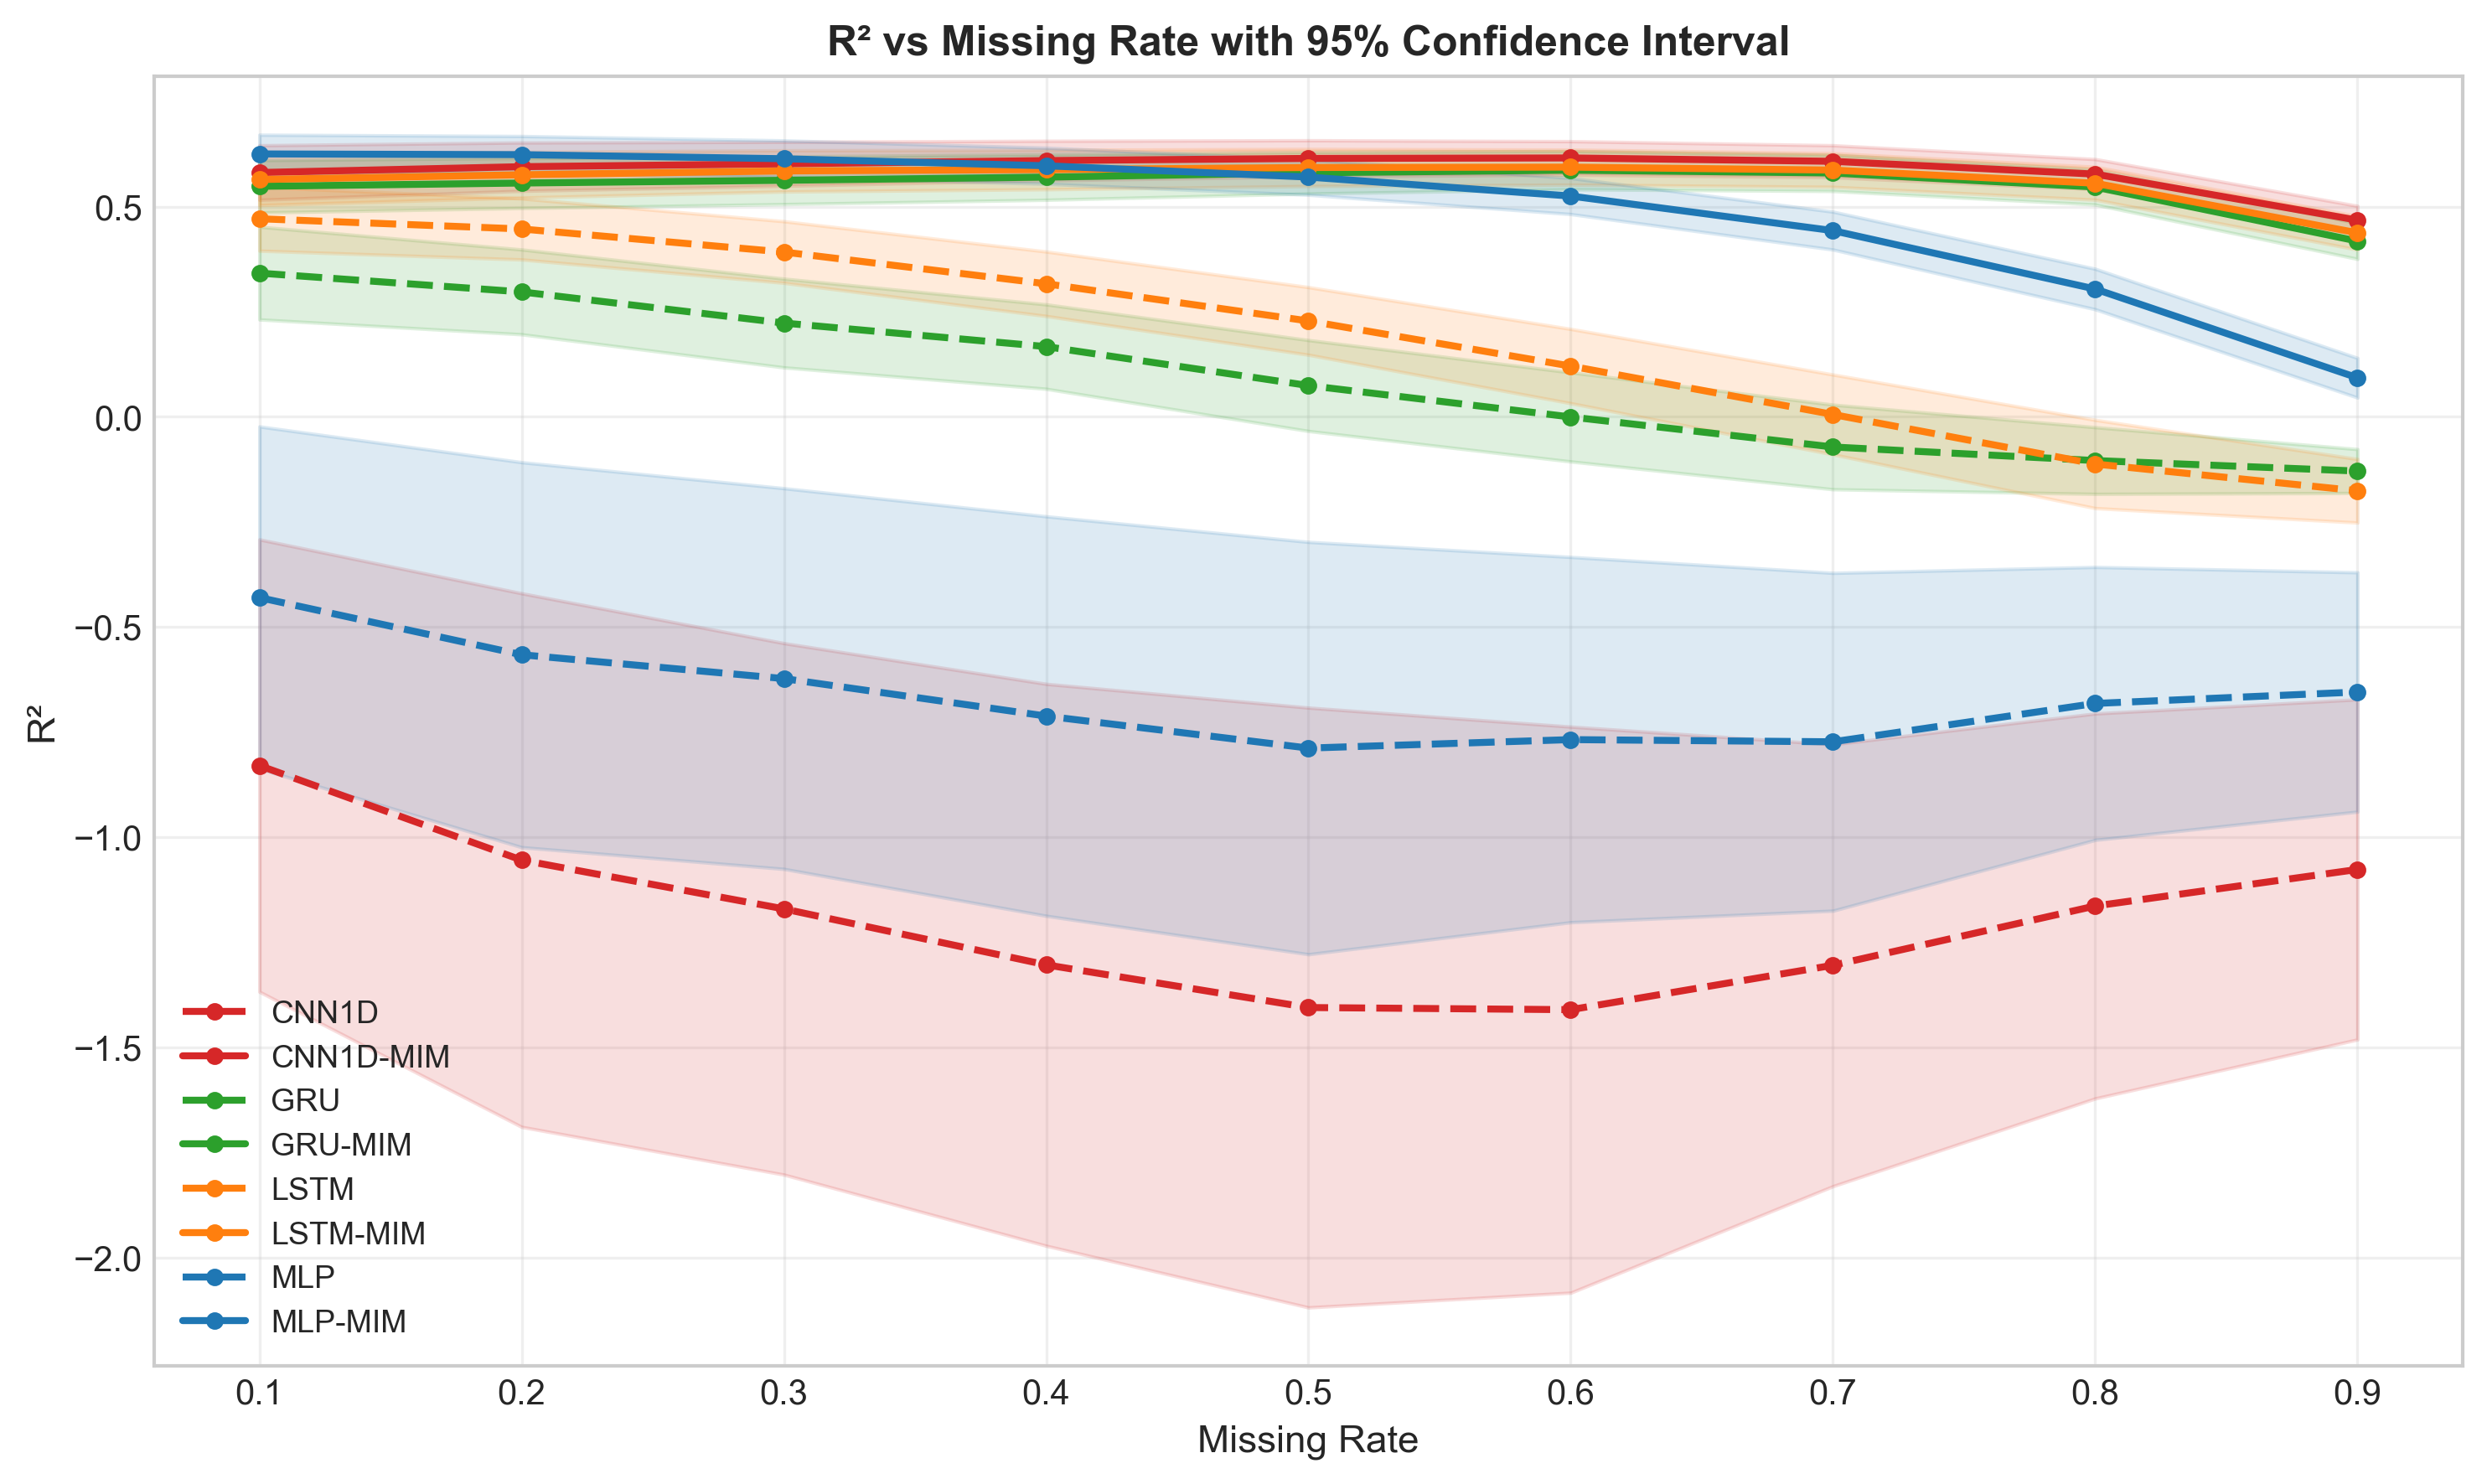
\includegraphics[width=\textwidth]{r2_curves_ci.png}
        \caption{R$^2$}
        \label{fig:r2_all}
    \end{subfigure}
    \caption{三种评价指标下的模型表现对比：(a) MAE；(b) RMSE；(c) R²。三种指标呈现一致的趋势，验证了MIM方法的有效性。}
    \label{fig:three_metrics}
\end{figure}

图\ref{fig:distribution}展示了不同缺失率下MAE的分布情况（小提琴图）。可以观察到，随着缺失率增加，基线模型的MAE分布逐渐向右偏移且展宽，表明不仅平均误差增大，而且稳定性下降；相比之下，MIM版本的分布中心始终保持在较低水平，且分布形态更为集中，说明MIM方法能够有效抑制高缺失率下的性能退化。

\begin{figure}[htbp]
    \centering
    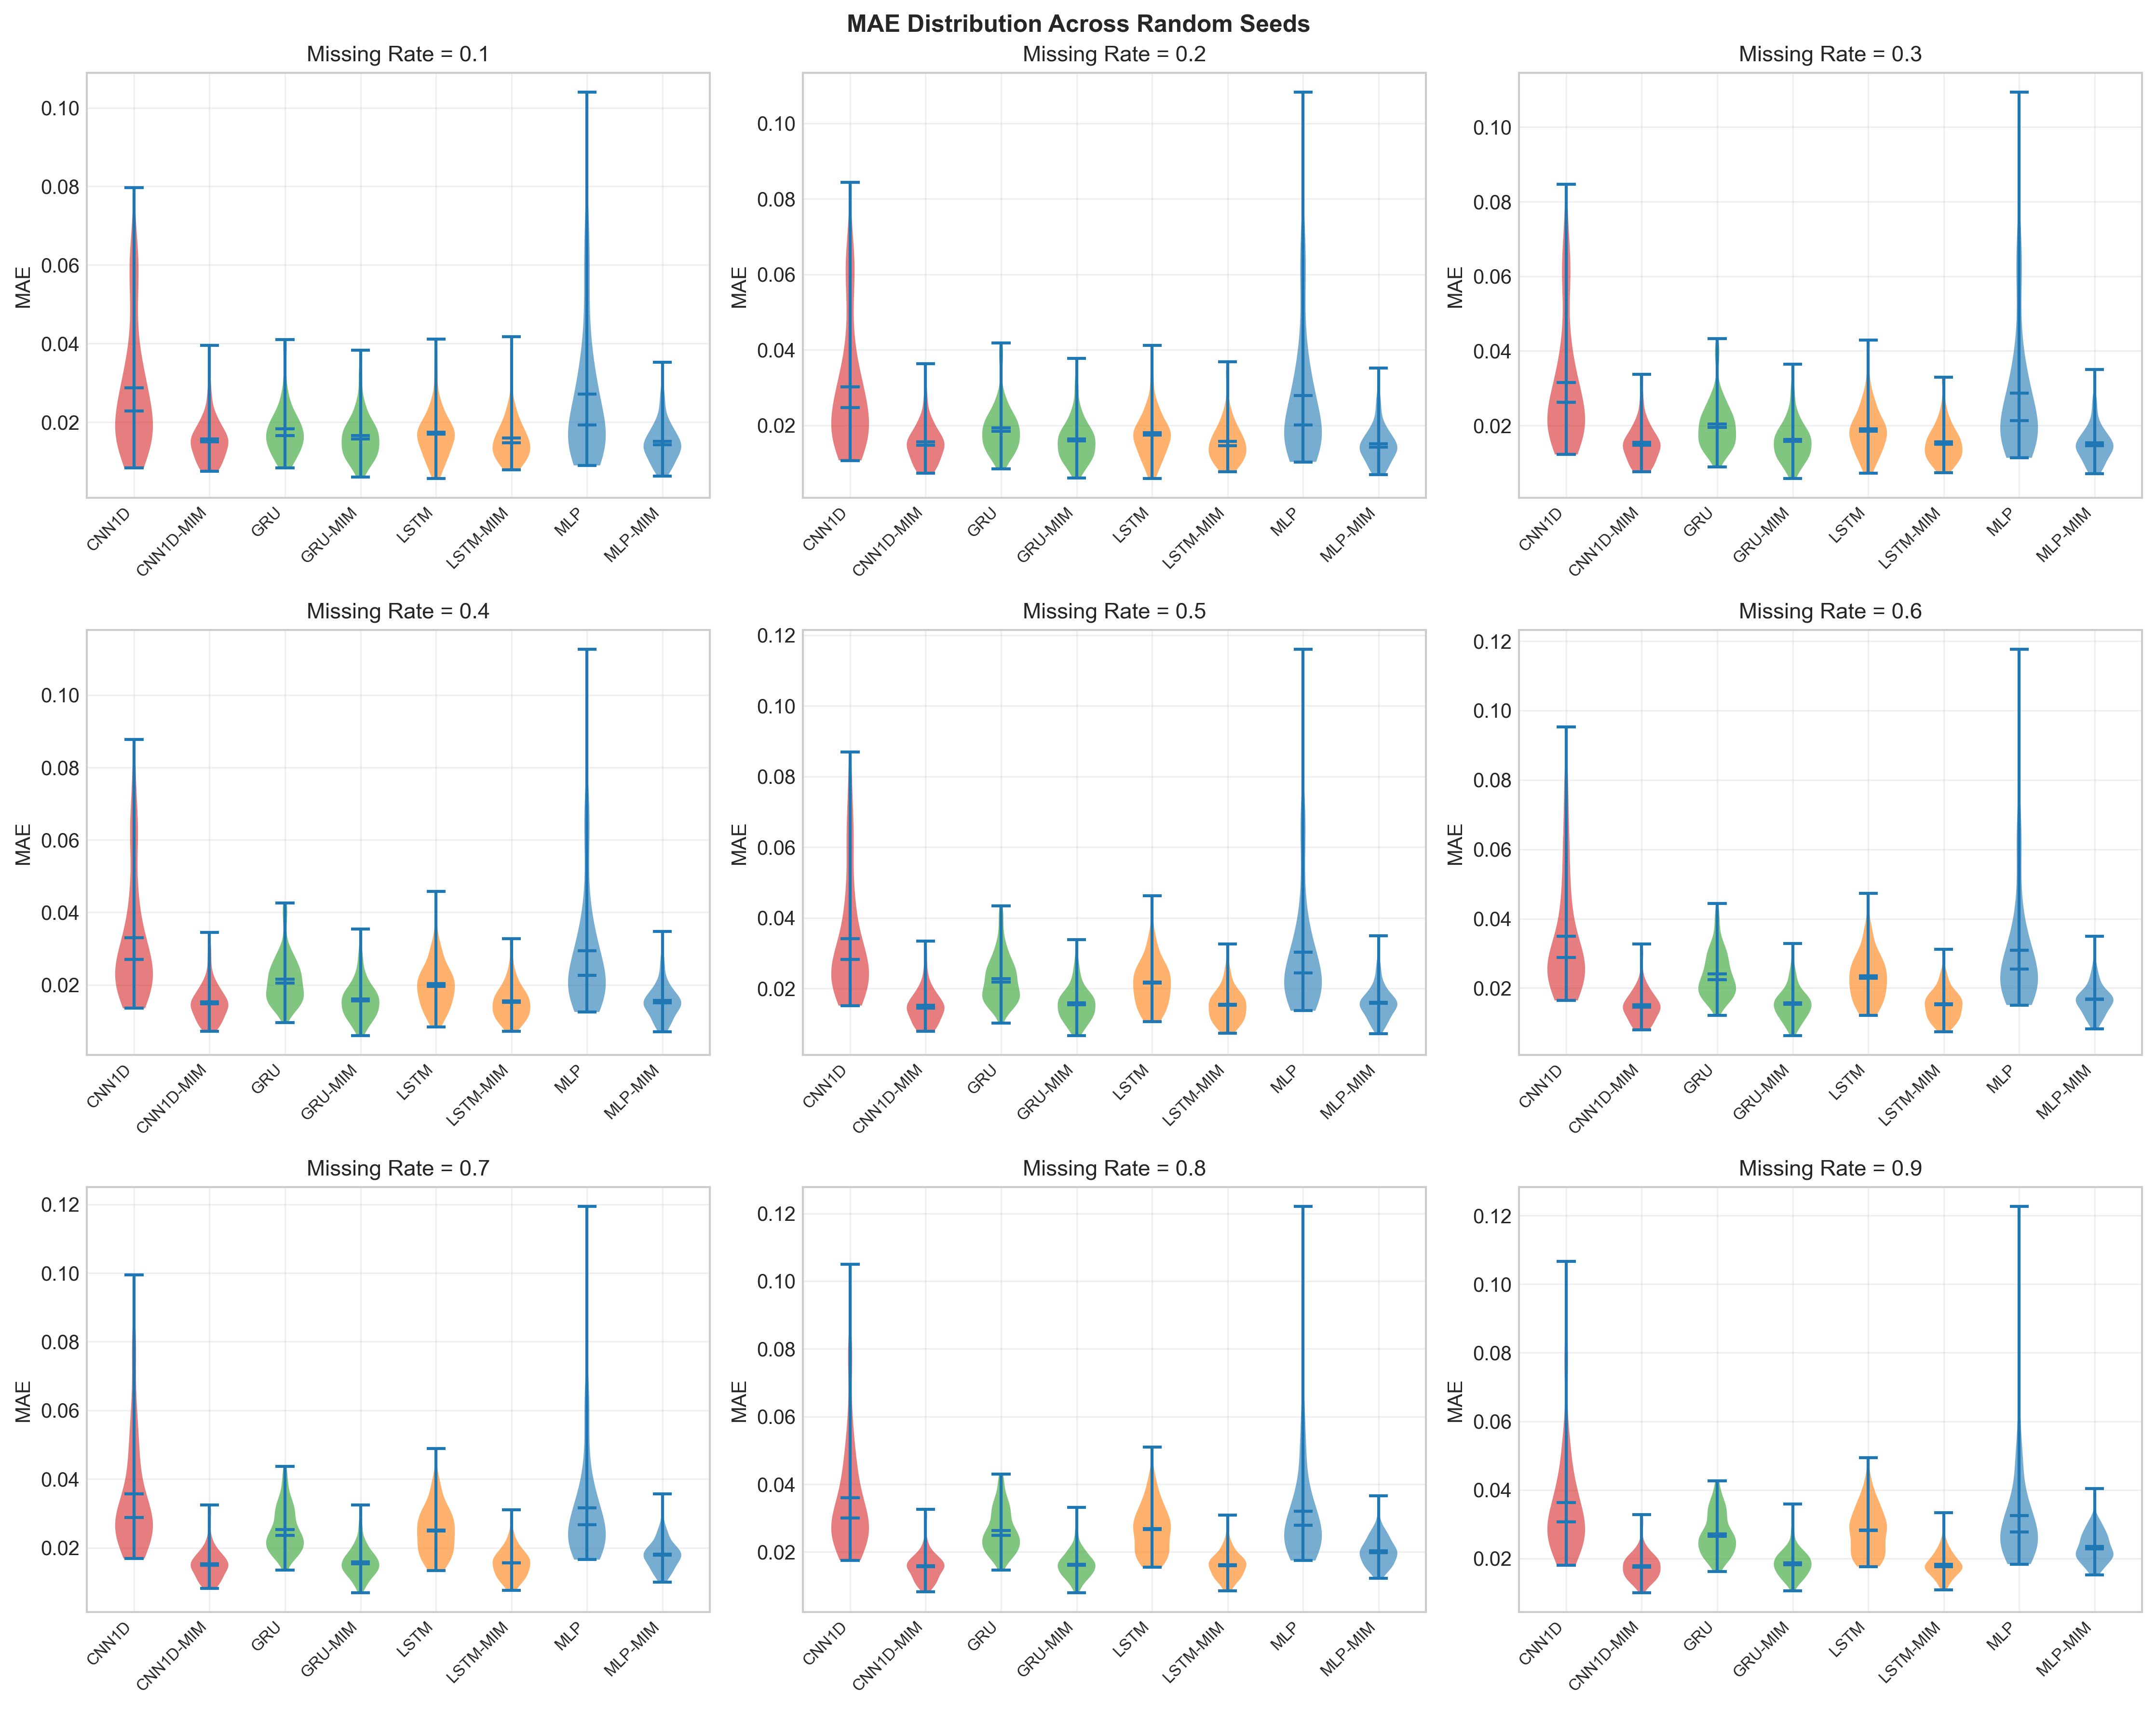
\includegraphics[width=0.95\textwidth]{mae_distribution.png}
    \caption{不同缺失率下MAE的分布情况（小提琴图）。每个子图对应一个缺失率，展示了各模型在该缺失率下的MAE分布密度。基线模型的分布随缺失率增加明显右偏，而MIM版本保持稳定。}
    \label{fig:distribution}
\end{figure}

%==============================================================================
\section{讨论}\label{sec:discussion}

\subsection{主要发现与机制分析}

基于上述实验结果，我们可以总结出三项主要发现，并对其背后的机制进行分析。

第一项发现是MIM方法在中高缺失率条件下对神经网络模型具有普遍的增益效果。当缺失率达到0.4及以上时，MLP、LSTM、GRU、1D-CNN四种神经网络架构均从MIM中获得显著的性能提升，改进率普遍超过50\%，在极端缺失（0.9）时甚至超过90\%。这一现象的机制可以从信息论的角度理解：在原始特征被大量缺失的情况下，插补值本身的信息含量大幅降低，甚至可能引入误导性的偏差；而缺失指示器提供了关于"哪些信息缺失"的元信息，这种元信息在缺失率较高时变得尤为珍贵——它告知模型哪些输入是可信的、哪些是估计的，使模型能够相应地调整对各特征的依赖程度。神经网络的多层非线性结构使其能够学习这种"可信度加权"机制，从而在输入层就将缺失信息纳入决策过程。

第二项发现是不同神经网络架构对MIM的利用效率存在差异，其中1D-CNN的增益最为显著（平均改进率93.9\%），而MLP相对较弱（平均改进率80.0\%）。从模型结构角度分析，1D-CNN通过时间轴上的卷积核聚合邻域信息，对输入特征的局部形状较为敏感。均值插补在时序维度上引入了平滑且缺乏物理意义的片段，使得卷积核难以区分"真实波形变化"与"填补伪迹"。MIM的二值指示向量在这一场景下提供了显式的"置信度"标签，使网络能够在特征融合时降低对被插补区域的依赖，因此在CNN结构中带来的相对收益更大。

相比之下，LSTM和GRU通过门控机制控制信息流，缺失指示器可以作为额外的门控信号，调节历史信息和当前输入的权重；而MLP作为全连接网络，特征之间缺乏结构性交互，可能难以充分利用缺失指示器提供的结构化信息。这一发现提示我们，MIM方法在不同神经网络架构上的价值存在差异，在具有局部感受野或门控机制的模型上效果更为突出。

\subsection{工程应用建议}

基于本研究的实验结果，我们为实际工程应用提出以下建议，以帮助工程师根据具体场景选择合适的模型和策略。

综合表\ref{tab:improvement_summary}的改进率和表\ref{tab:full_results}的MAE/RMSE/R²结果，在不同缺失率区间可给出以下工程建议：

（1）在缺失率较低（MR$\leq$0.3）且计算资源有限的场景下，基线模型已能取得较小误差（例如MLP-Baseline在MR=0.1时MAE$\approx$0.089，RMSE$\approx$0.121），此时是否引入MIM需视部署复杂度而定。若资源极度受限且缺失率确实较低，可采用简单MLP基线模型。

（2）在中等缺失率（0.3$<$MR$\leq$0.6）时，MLP-MIM和GRU-MIM在保持较低参数量的同时，实现了75\%--86\%的MAE相对改进（如MR=0.5时，MLP-MIM将MAE从0.189降至0.029，GRU-MIM从0.098降至0.014），适合作为通用部署方案。GRU-MIM参数量适中（约40,000--44,000），能够利用时序信息，适合需要连续预测SOH序列的应用。

（3）在高缺失率（MR$\geq$0.7）或关键应用场景下，1D-CNN-MIM的平均改进率可达93.9\%，在MR=0.9时仍能将MAE维持在约0.020水平，而基线模型MAE普遍超过0.2。1D-CNN-MIM在性能-参数量效率方面表现最优（Baseline约16,700参数，MIM版本约21,300参数），是资源充足场景下的首选方案。

\subsection{局限性与未来工作}

本研究虽然在多模型、多缺失率条件下系统评估了MIM方法，但仍存在一些局限性值得在未来工作中改进。

首先，在缺失机制方面，本研究仅考虑了完全随机缺失（MCAR），即缺失位置与任何观测或未观测变量都无关。然而，实际工程中更常见的是随机缺失（MAR）或非随机缺失（MNAR）——例如，老化程度较高的电池可能更容易出现传感器故障，导致缺失与SOH本身相关。不同缺失机制下MIM的效果可能存在差异，未来工作应扩展至MAR和MNAR场景的验证。

其次，在数据集方面，本研究仅使用了XJTU单一数据集进行验证，虽然该数据集涵盖了多种工况和电池类型，但仍缺乏对其他公开数据集（如NASA、CALCE、Oxford等）的跨数据集验证。未来应在更多数据集上验证MIM方法的泛化能力，并探索跨数据集迁移学习的可能性。

最后，在插补方法方面，本研究仅采用了最简单的均值插补作为基础。虽然实验结果表明"是否使用MIM"比"使用哪种插补"更关键，但系统对比其他插补方法（如前向填充、线性插值、矩阵分解等）与MIM的组合效果仍是有价值的研究方向。此外，与纯数据驱动方法相比，将电化学机理知识通过物理信息神经网络（PINN）融入模型，有望在数据稀缺和工况迁移时进一步提升SOH预测的稳定性与可解释性\cite{wang2024pinn}。

%==============================================================================
\section{结论}\label{sec:conclusion}

本文针对电池健康状态（SOH）预测中的数据缺失问题，系统评估了缺失指示器方法（MIM）在多种常用模型架构和不同缺失率条件下的有效性。基于XJTU数据集的实验结果表明，MIM方法在神经网络模型上能够显著提升中高缺失率场景下的SOH预测性能，为实际电池管理系统中的缺失数据处理提供了一种简洁而有效的技术方案。

本文的主要结论可以概括为以下四点：（1）在九档缺失率（$\{0.1, 0.2, \ldots, 0.9\}$）条件下的系统实验表明，MIM方法在MLP、LSTM、GRU、1D-CNN等深度学习模型架构中普遍带来SOH预测性能提升，在MR$\geq 0.4$条件下改进率可达50\%--96\%（如1D-CNN-MIM在MR=0.5时改进率达96.1\%），验证了缺失指示器在电池SOH预测领域的应用价值。（2）不同模型架构从MIM获益的程度存在差异，1D-CNN和时序模型（LSTM、GRU）的增益最为显著；但总体而言，"有MIM的深度学习模型"比"无MIM的对应模型"更鲁棒，在100个随机种子下表现出更低的MAE均值和更小的方差（$p<$0.001）。（3）在基础插补方法（均值插补）固定的情况下，影响SOH预测性能的首要因素是"是否使用缺失指示器"，而非具体选用哪一种基础插补方法，这一发现对于工程实践具有指导意义——在资源有限时，应优先实现MIM而非追求复杂的插补算法。（4）基于实验数据，本文给出了分场景的模型选择建议：MR$\leq$0.3时基线模型已能满足需求；0.3$<$MR$\leq$0.6时推荐MLP-MIM或GRU-MIM（改进率75\%--86\%）；MR$\geq$0.7时推荐1D-CNN-MIM（改进率$>$90\%，参数量仅约21,300）。

面向工程部署的电池健康管理，除点估计误差外，置信区间与不确定性量化同样关键\cite{geng2025uqsoh}。在工程应用中，SOH点估计之外的置信区间同样重要，已有工作通过贝叶斯或自助法实现不确定性量化，为运维决策提供风险感知能力\cite{geng2025uqsoh}。本研究在报告MAE/RMSE的同时给出了95\%置信区间，为实际应用提供了更全面的可靠性评估。本研究为数据驱动的电池SOH预测方法在实际工程环境中的应用提供了有价值的实证依据和技术指导。未来工作将扩展至非随机缺失机制、跨数据集验证以及与其他先进插补方法的联合应用等方向。

%==============================================================================
\bibliographystyle{unsrtnat}
\bibliography{references}

\end{document}
